\documentclass{article}
\usepackage{graphicx} %package to manage images
\usepackage[utf8]{inputenc}
\usepackage[a4paper, total={6in, 8in}]{geometry}
\usepackage{xurl}
\usepackage{hyperref}
\usepackage{float}
\title{Relatório 13 \\ ROC curves}
\author{Pedro A. S. O. Neto}
\date{Setembro, 2023}

\begin{document}

\maketitle

\section{Final ANOVAS}

Descriptive of the sample. 

\begin{table}[ht]
\centering
\begin{tabular}{rllrrr}
  \hline
 & sexo & tea & sdAgeJA & meanAgeJA & N \\ 
  \hline
1 & F & TD & 1.00 & 2.89 & 188 \\ 
  2 & F & TEA &  & 2.00 &   1 \\ 
  3 & F & nonTD & 0.83 & 3.03 &   5 \\ 
  4 & F & other & 1.59 & 2.54 &   2 \\ 
  5 & F &  & 1.06 & 3.38 &   4 \\ 
  6 & M & TD & 1.04 & 2.78 & 203 \\ 
  7 & M & TEA & 0.84 & 2.93 &  22 \\ 
  8 & M & nonTD & 0.69 & 3.48 &   8 \\ 
  9 & M & other & 0.74 & 3.15 &   4 \\ 
  10 & M &  & 0.83 & 3.05 &   7 \\ 
  11 & nan &  &  &  &   3 \\ 
   \hline
\end{tabular}
\end{table}

\begin{figure}[H]
  \caption{ANOVA alternancias}
  \noindent\makebox[\textwidth]{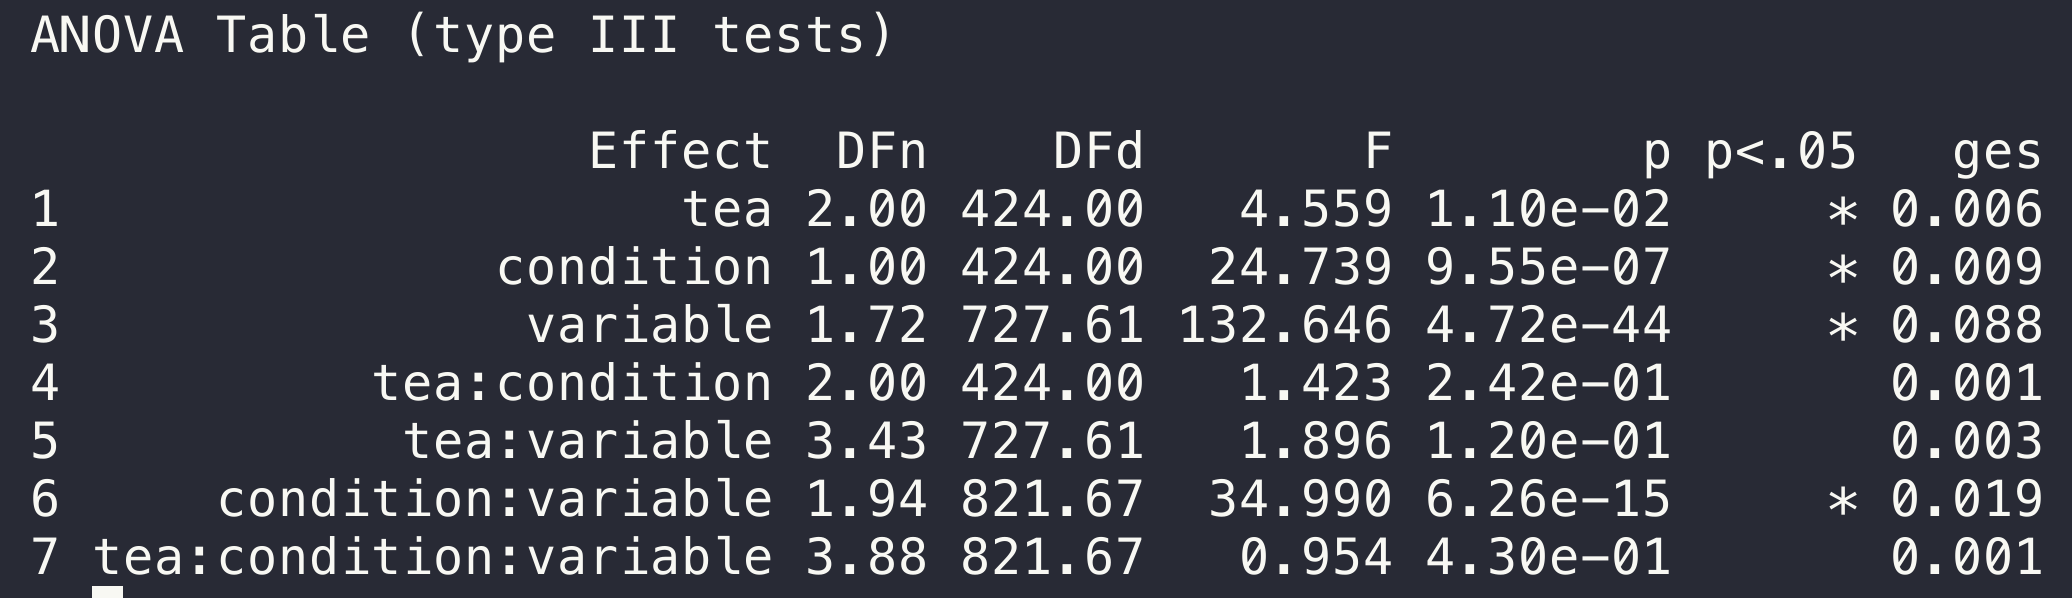
\includegraphics[scale=0.5]{./anovaAlternancia.png}}
  \centering
\end{figure}

\begin{figure}[H]
  \caption{Main effect of TEA on alternancia}
  \noindent\makebox[\textwidth]{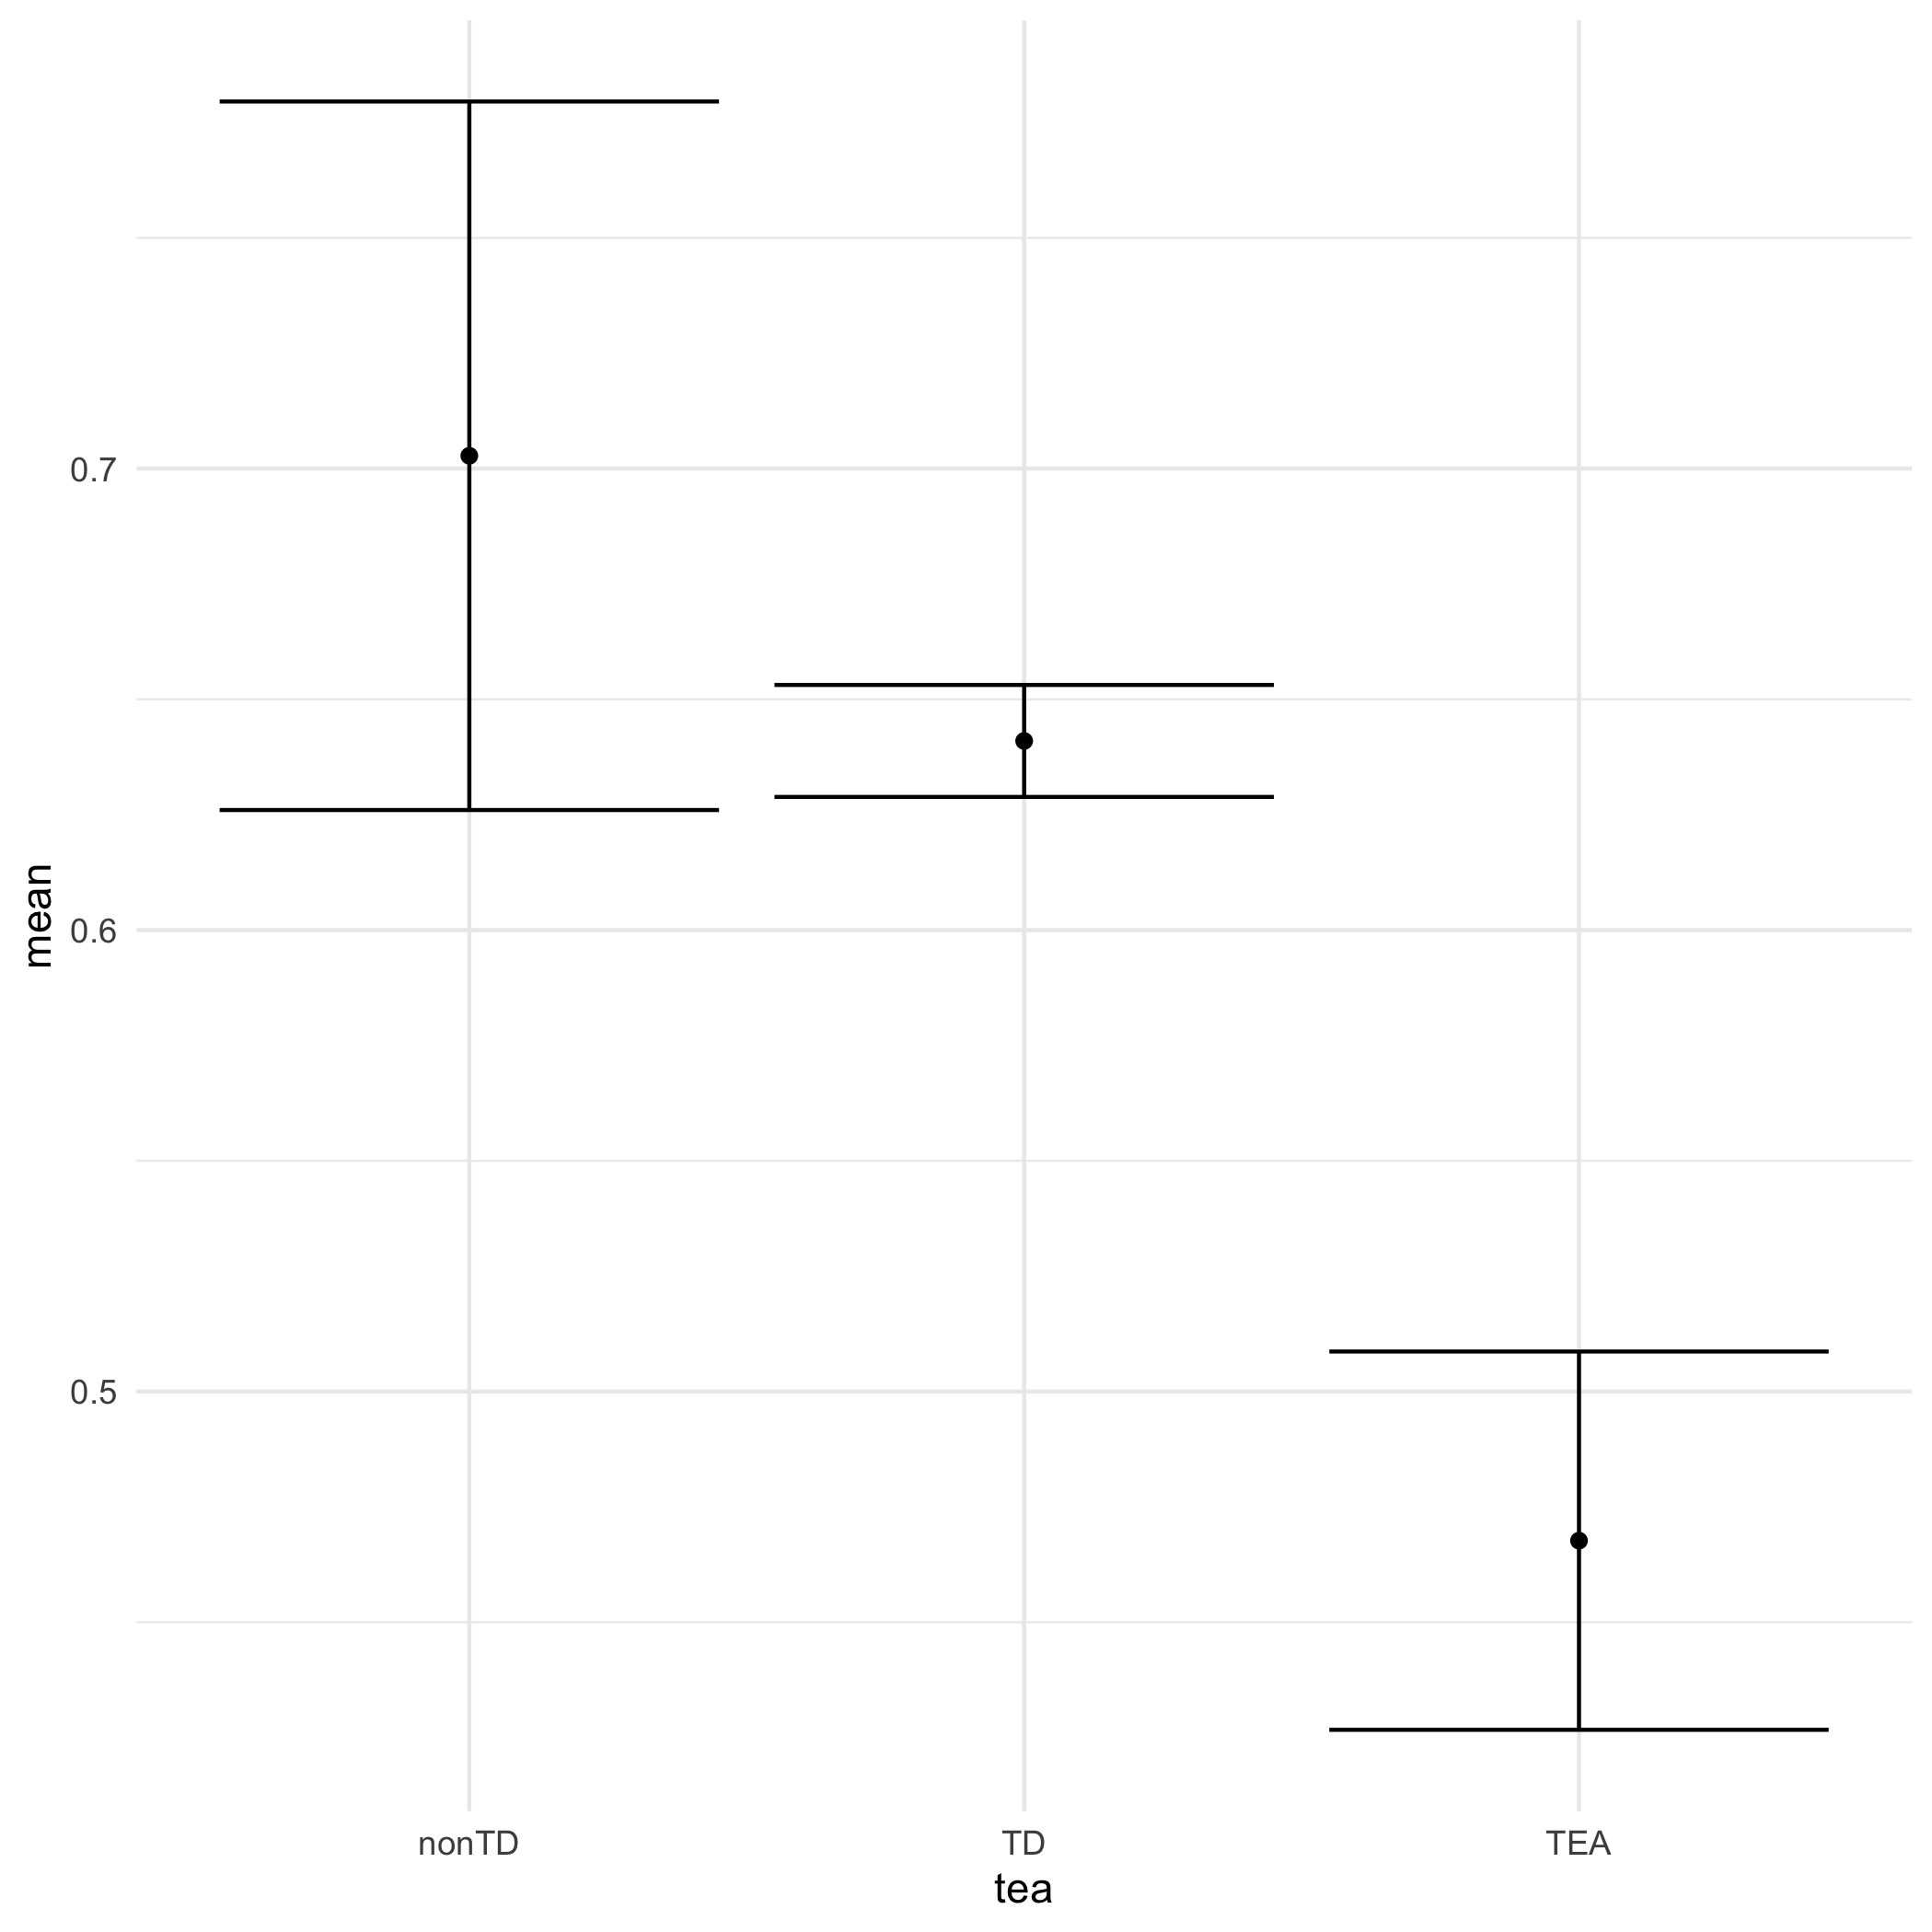
\includegraphics[scale=0.2]{./teaMainAlternancia.png}}
  \centering
\end{figure}

\begin{table}[ht]
\centering
\caption{Main effect of TEA on alternancia}
\begin{tabular}{rlrr}
  \hline
 & tea & mean & stder \\ 
  \hline
1 & nonTD & 0.70 & 0.08 \\ 
  2 & TD & 0.64 & 0.01 \\ 
  3 & TEA & 0.47 & 0.04 \\ 
   \hline
\end{tabular}
\end{table}

\begin{figure}[H]
  \caption{Main effect of variable on alternancia}
  \noindent\makebox[\textwidth]{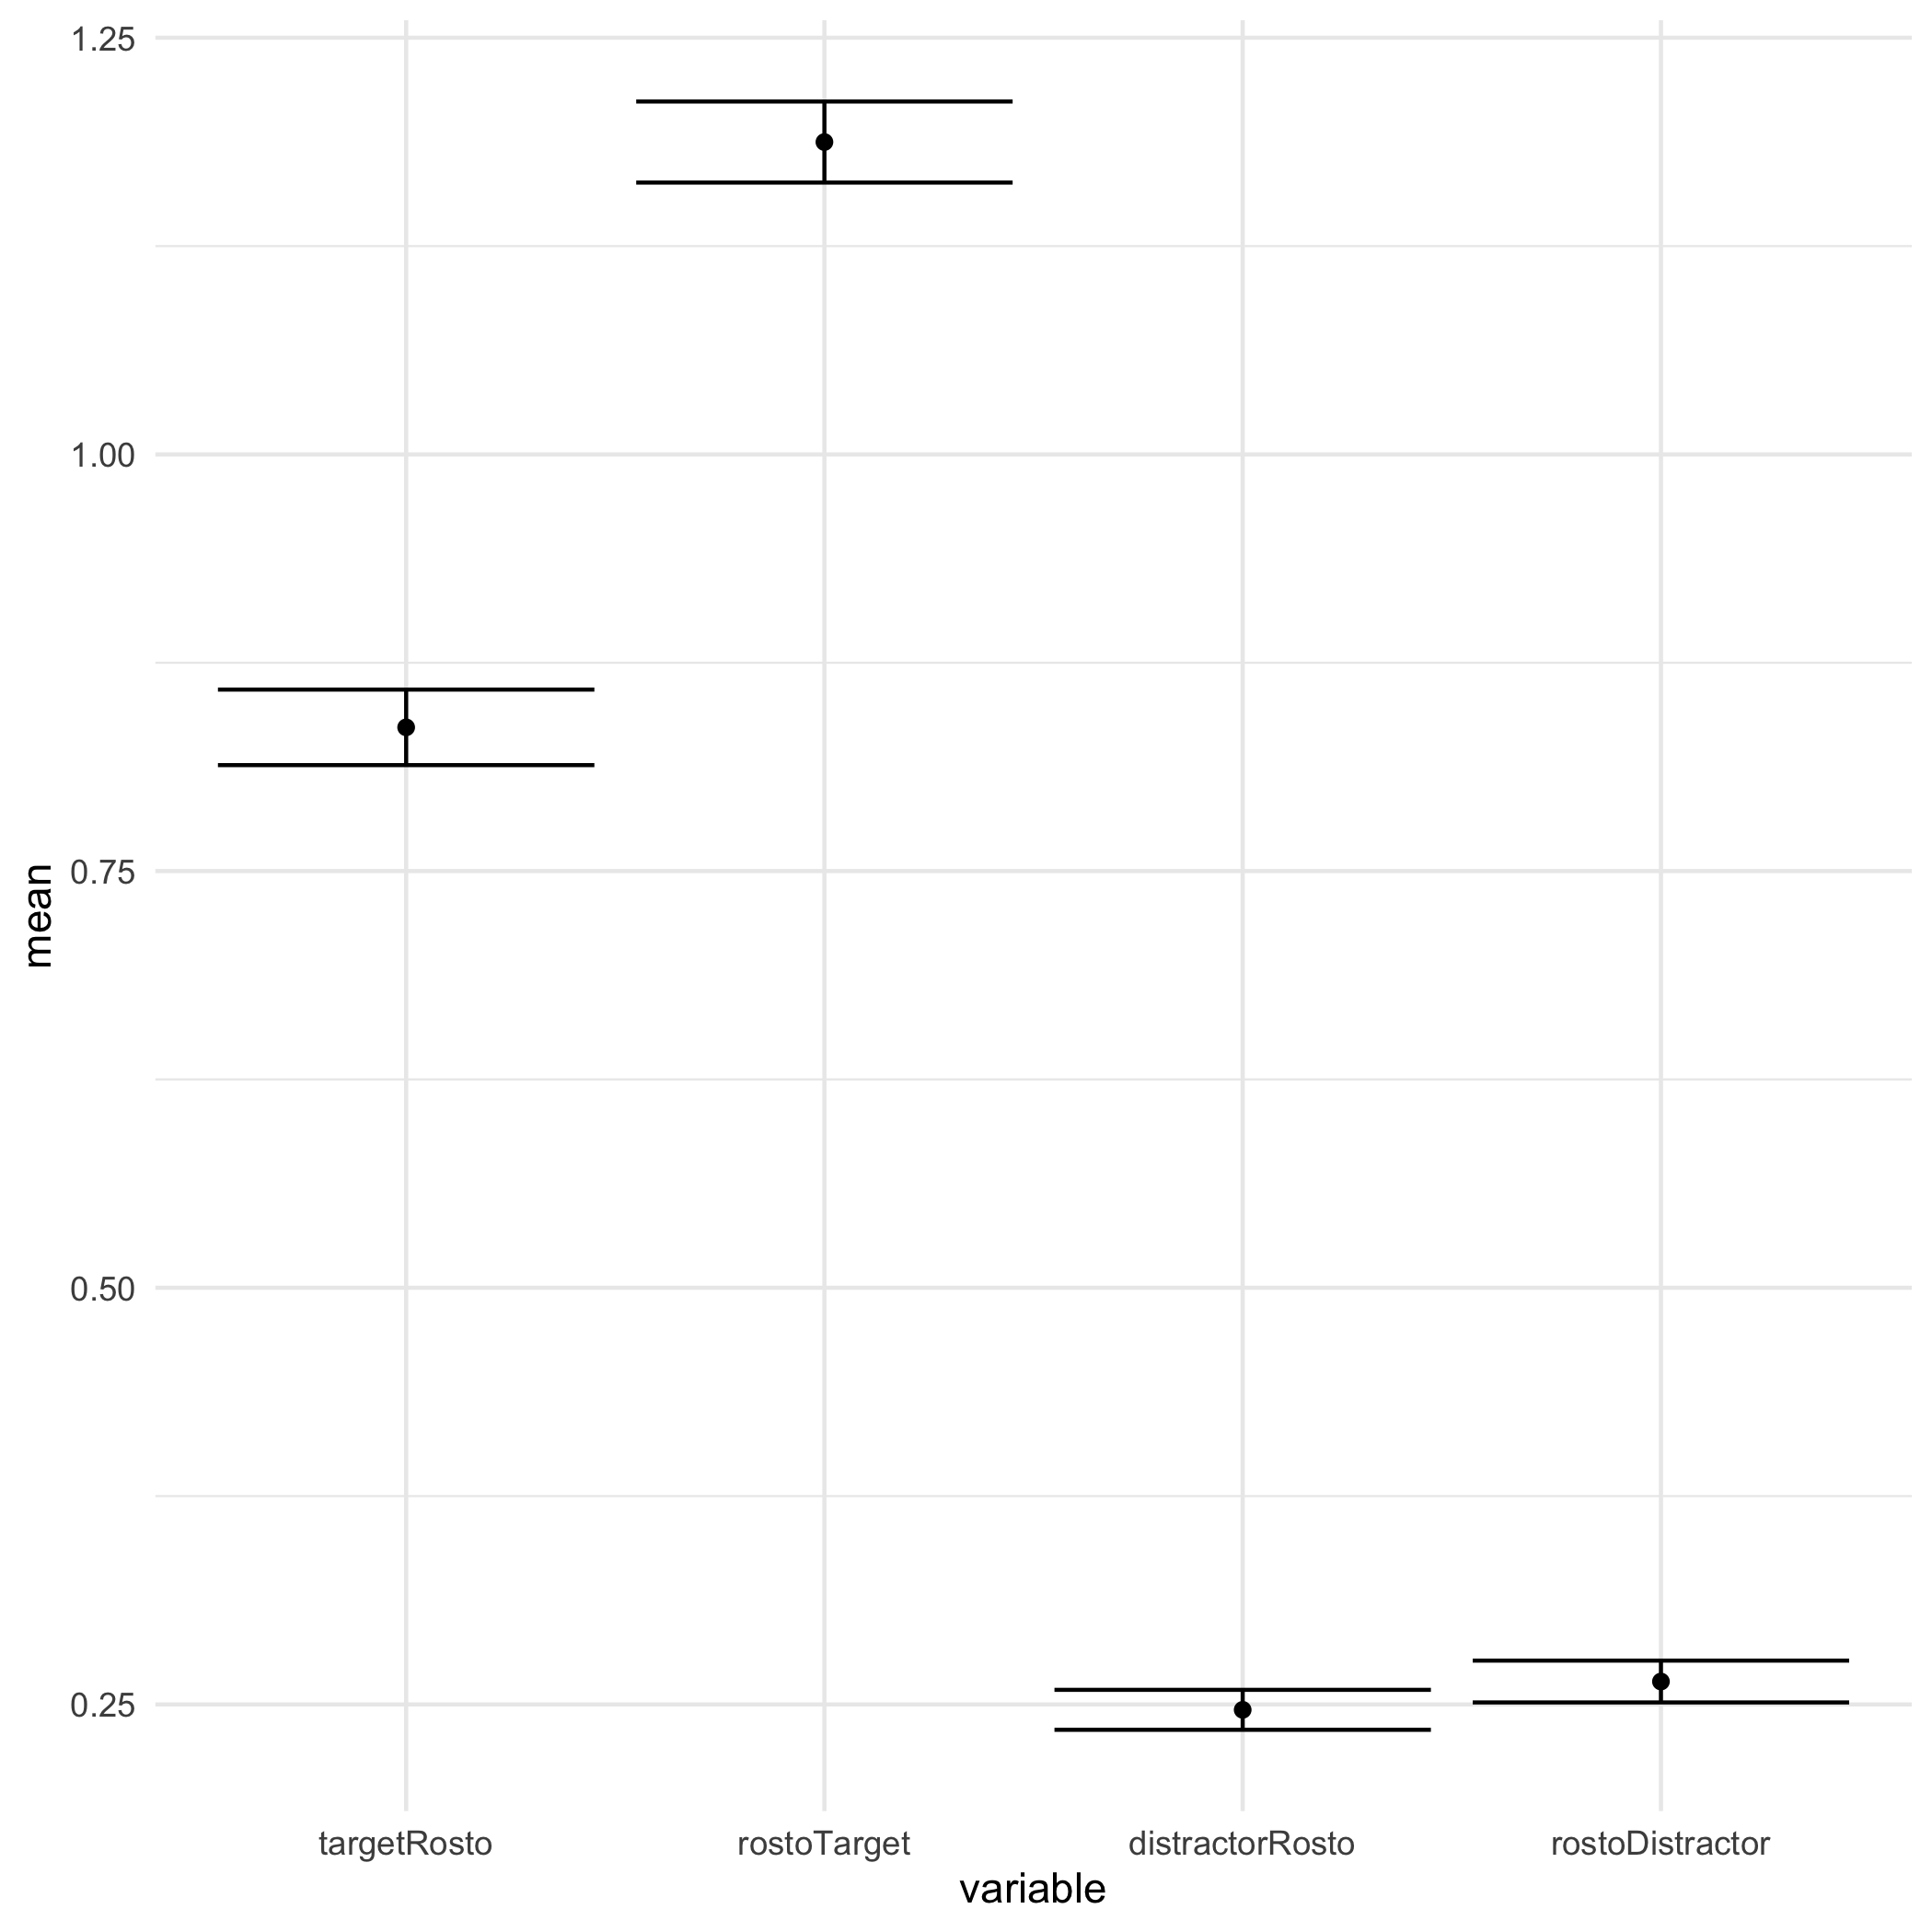
\includegraphics[scale=0.2]{./alternanciaVariable.png}}
  \centering
\end{figure}

\begin{table}[ht]
\caption{Main effect of variable on alternancia}
\centering
\begin{tabular}{rlrr}
  \hline
 & variable & mean & stder \\ 
  \hline
  1 & targetRosto & 0.84 & 0.02 \\ 
  2 & rostoTarget & 1.19 & 0.02 \\ 
  3 & distractorRosto & 0.25 & 0.01 \\ 
  4 & rostoDistractor & 0.26 & 0.01 \\ 
   \hline
\end{tabular}
\end{table}

\begin{figure}[H]
  \caption{Interaction of condition and variable on alternancia}
  \noindent\makebox[\textwidth]{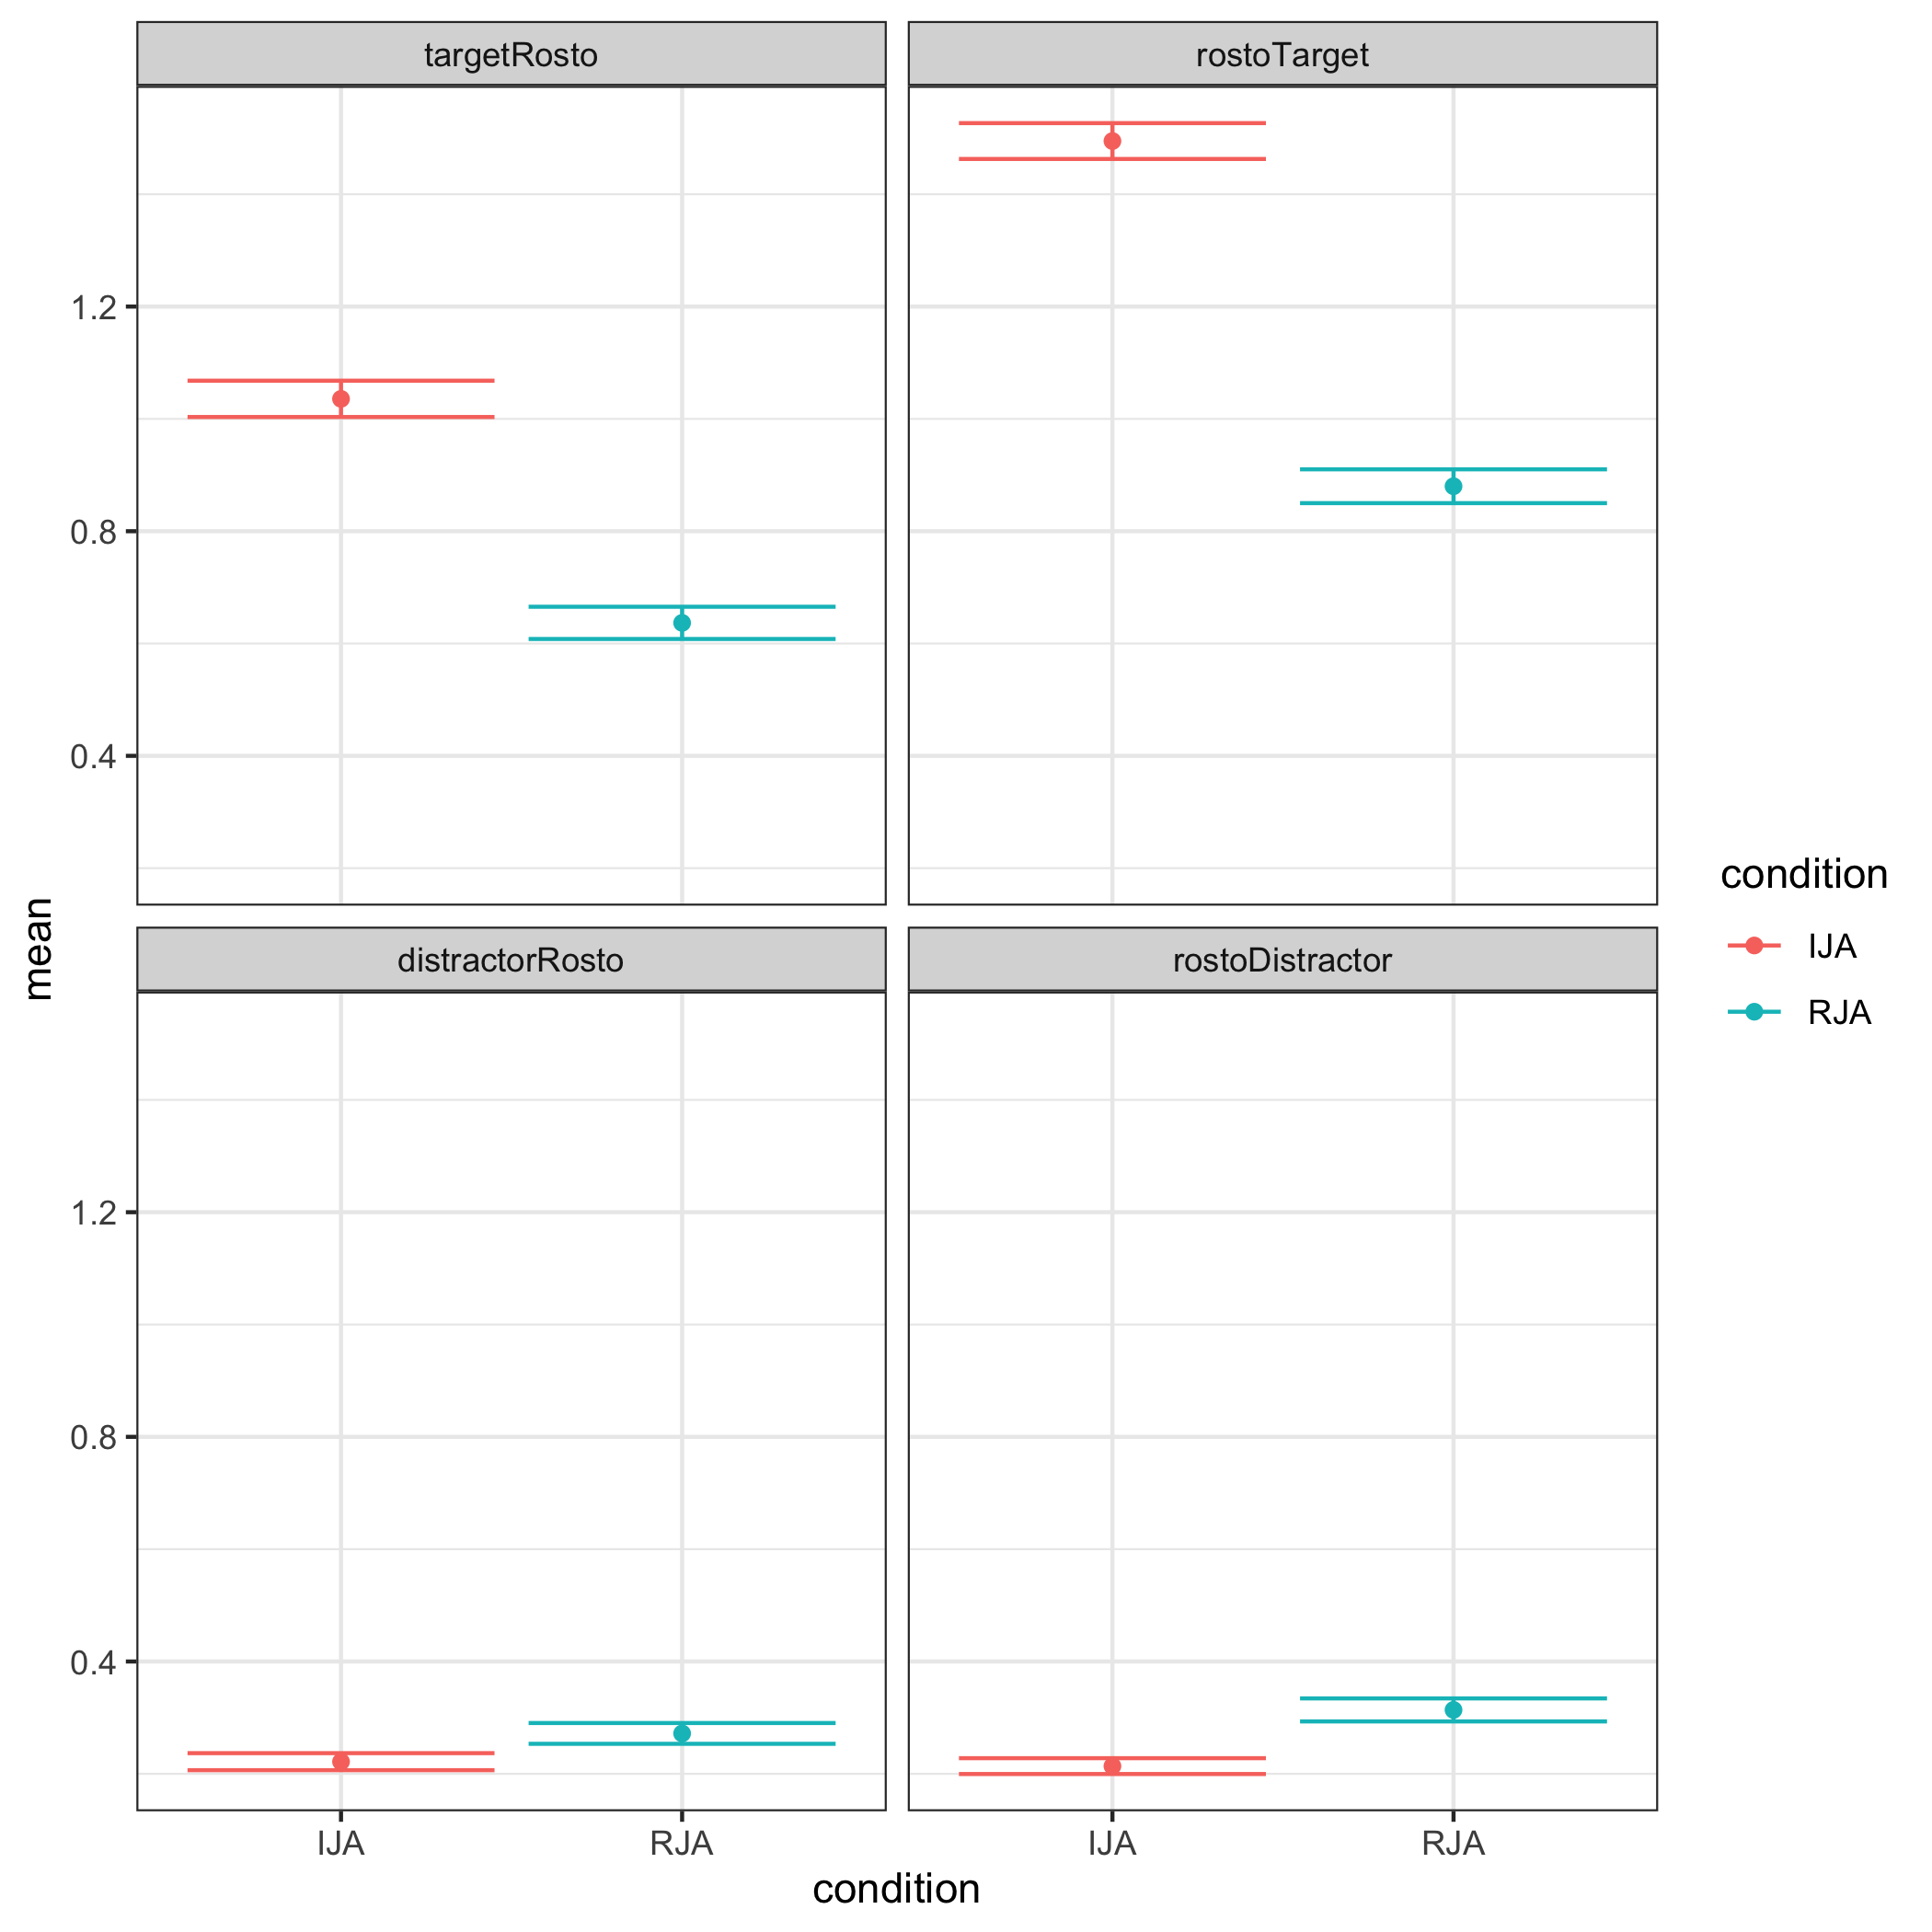
\includegraphics[scale=0.2]{./conditionVariable.png}}
  \centering
\end{figure}

\begin{table}[ht]
\centering
\caption{Interaction of condition and variable on alternancia}
\begin{tabular}{rllrr}
  \hline
 & condition & variable & mean & stder \\ 
  \hline
1 & IJA & targetRosto & 1.04 & 0.03 \\ 
  2 & IJA & rostoTarget & 1.49 & 0.03 \\ 
  3 & IJA & distractorRosto & 0.22 & 0.02 \\ 
  4 & IJA & rostoDistractor & 0.21 & 0.01 \\ 
  5 & RJA & targetRosto & 0.64 & 0.03 \\ 
  6 & RJA & rostoTarget & 0.88 & 0.03 \\ 
  7 & RJA & distractorRosto & 0.27 & 0.02 \\ 
  8 & RJA & rostoDistractor & 0.31 & 0.02 \\ 
   \hline
\end{tabular}
\end{table}


\begin{figure}[H]
  \caption{Interaction of condition, variable and TEA. *Not statistically significant.}
  \noindent\makebox[\textwidth]{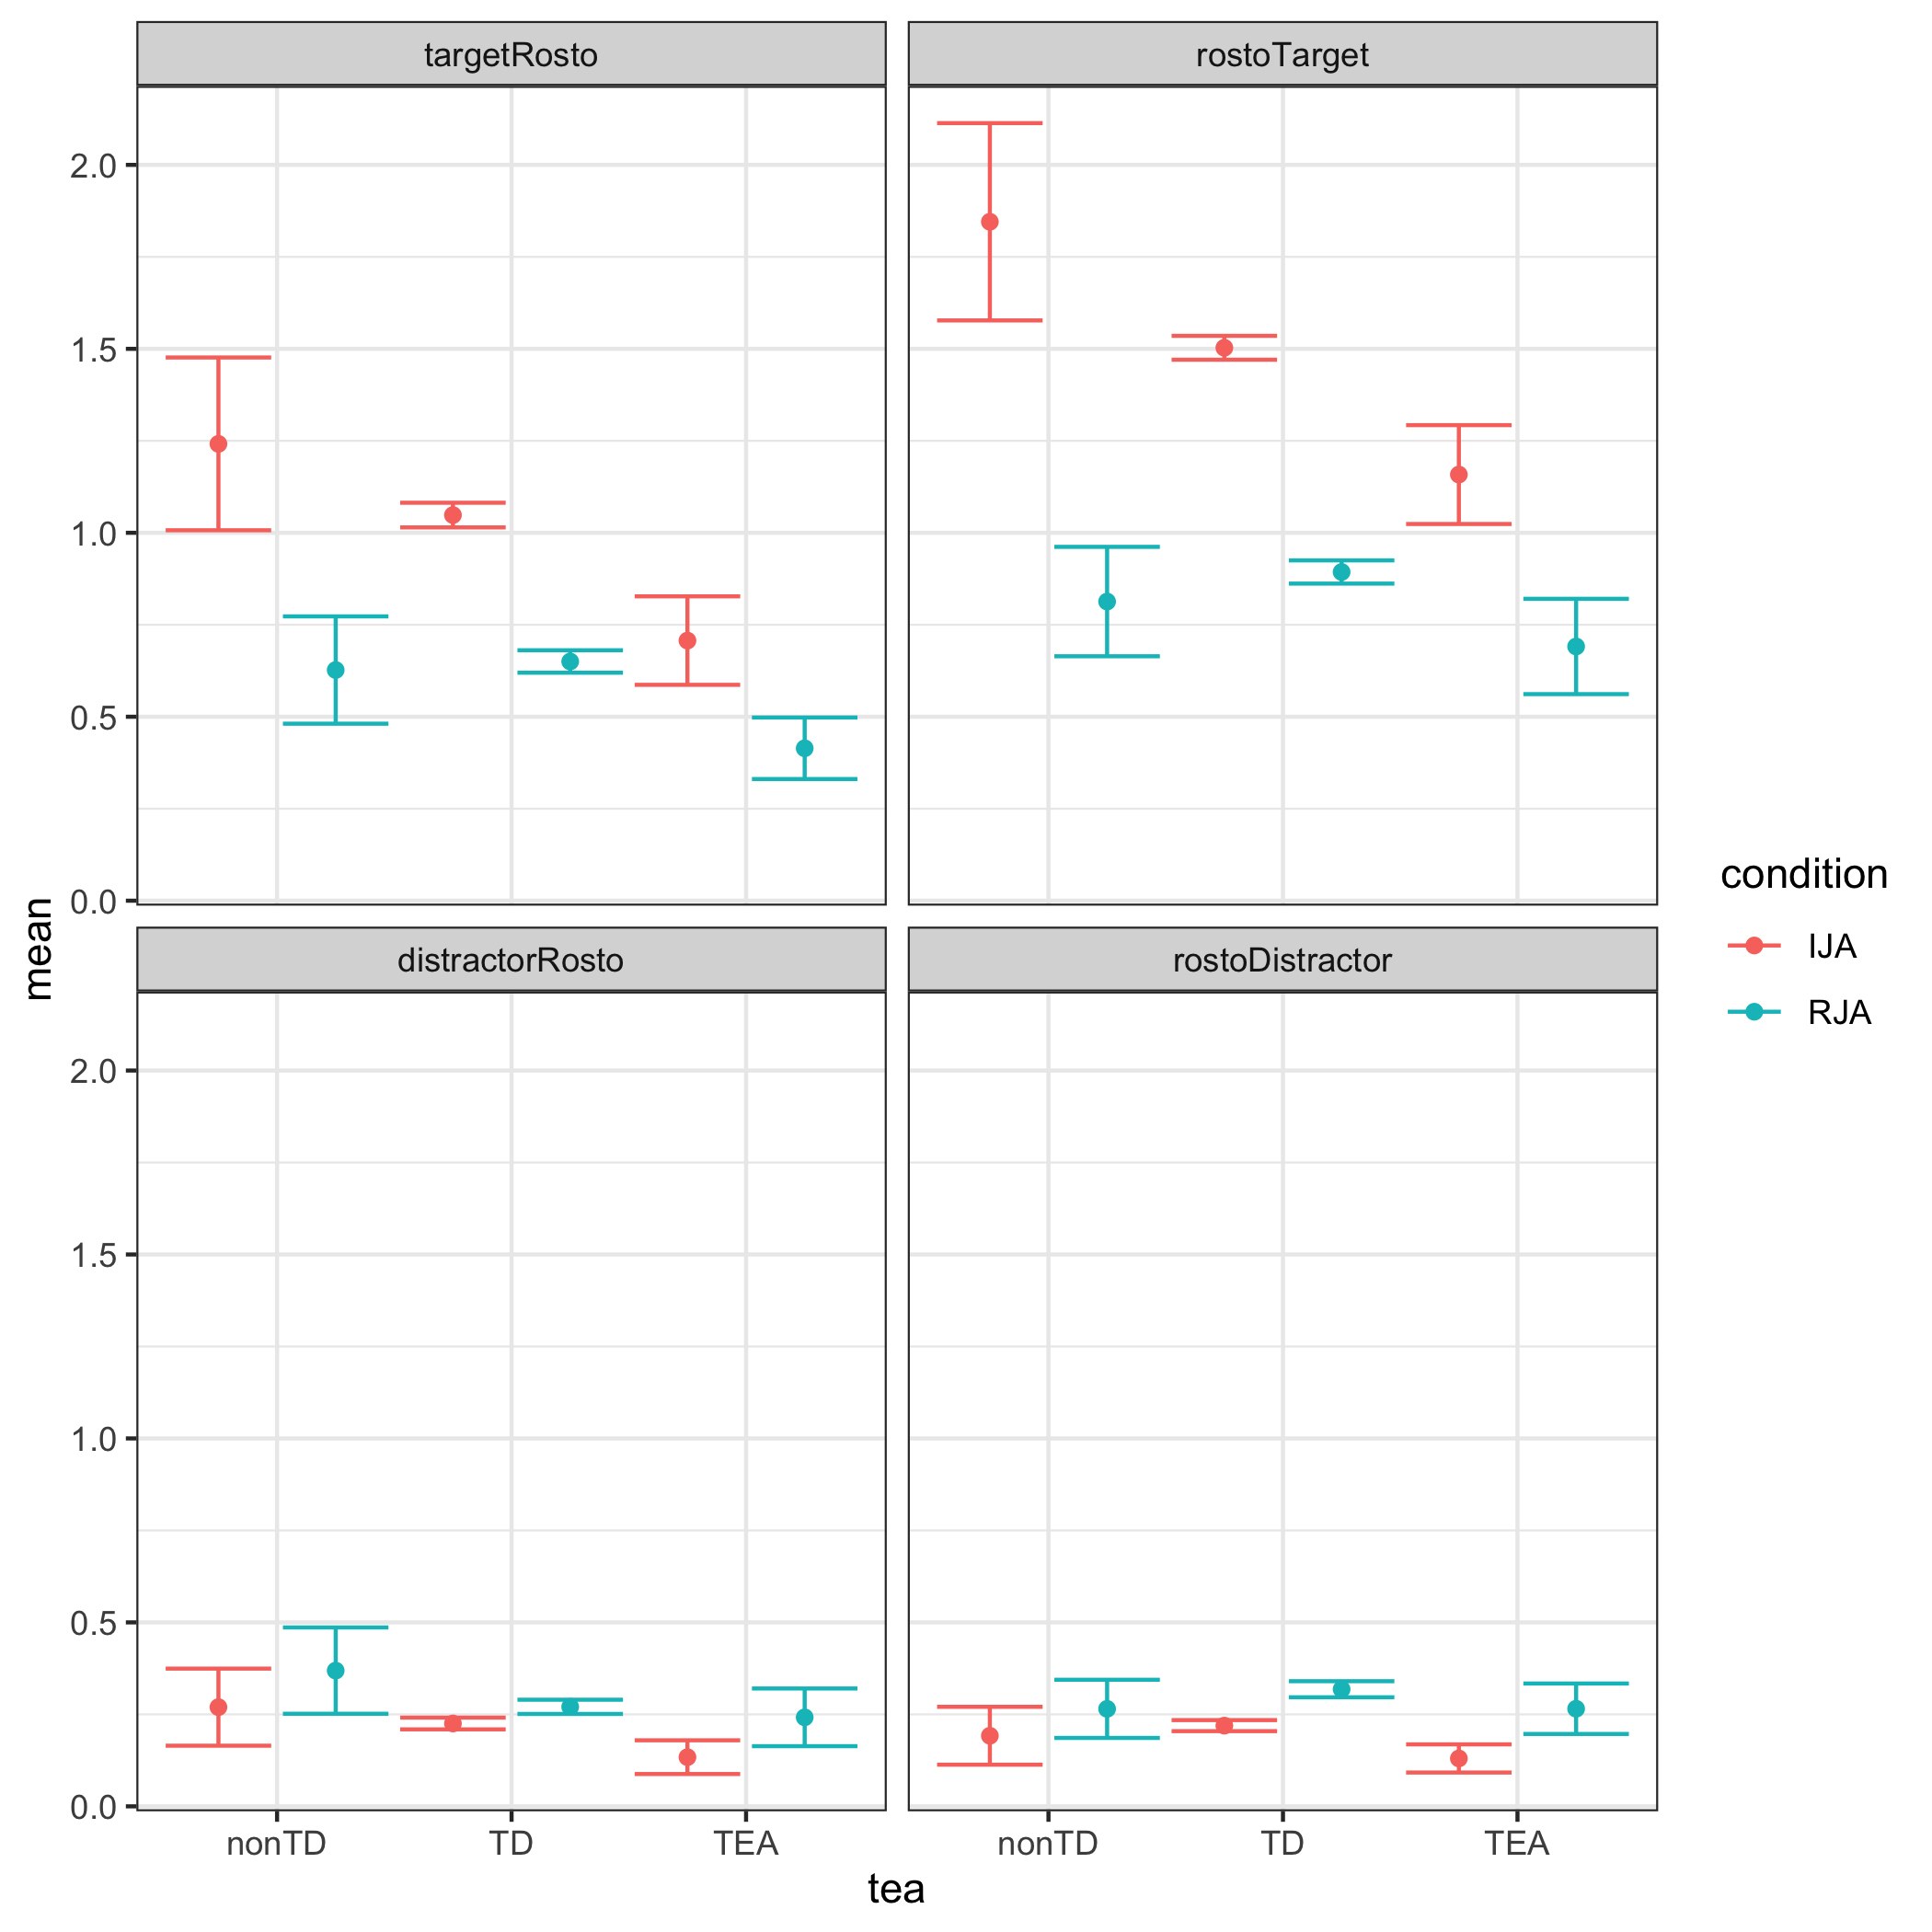
\includegraphics[scale=0.2]{./conditionVariableTea.png}}
  \centering
\end{figure}


\begin{table}[ht]
\centering
\caption{Interaction of condition, variable and TEA. *Not statistically significant.}
\begin{tabular}{rlllrr}
  \hline
 & condition & variable & tea & mean & stder \\ 
  \hline
1 & IJA & targetRosto & nonTD & 1.24 & 0.23 \\ 
  2 & IJA & targetRosto & TD & 1.05 & 0.03 \\ 
  3 & IJA & targetRosto & TEA & 0.71 & 0.12 \\ 
  4 & IJA & rostoTarget & nonTD & 1.85 & 0.27 \\ 
  5 & IJA & rostoTarget & TD & 1.50 & 0.03 \\ 
  6 & IJA & rostoTarget & TEA & 1.16 & 0.13 \\ 
  7 & IJA & distractorRosto & nonTD & 0.27 & 0.10 \\ 
  8 & IJA & distractorRosto & TD & 0.23 & 0.02 \\ 
  9 & IJA & distractorRosto & TEA & 0.13 & 0.05 \\ 
  10 & IJA & rostoDistractor & nonTD & 0.19 & 0.08 \\ 
  11 & IJA & rostoDistractor & TD & 0.22 & 0.01 \\ 
  12 & IJA & rostoDistractor & TEA & 0.13 & 0.04 \\ 
  13 & RJA & targetRosto & nonTD & 0.63 & 0.15 \\ 
  14 & RJA & targetRosto & TD & 0.65 & 0.03 \\ 
  15 & RJA & targetRosto & TEA & 0.41 & 0.08 \\ 
  16 & RJA & rostoTarget & nonTD & 0.81 & 0.15 \\ 
  17 & RJA & rostoTarget & TD & 0.89 & 0.03 \\ 
  18 & RJA & rostoTarget & TEA & 0.69 & 0.13 \\ 
  19 & RJA & distractorRosto & nonTD & 0.37 & 0.12 \\ 
  20 & RJA & distractorRosto & TD & 0.27 & 0.02 \\ 
  21 & RJA & distractorRosto & TEA & 0.24 & 0.08 \\ 
  22 & RJA & rostoDistractor & nonTD & 0.26 & 0.08 \\ 
  23 & RJA & rostoDistractor & TD & 0.32 & 0.02 \\ 
  24 & RJA & rostoDistractor & TEA & 0.27 & 0.07 \\ 
   \hline
\end{tabular}
\end{table}



\begin{figure}[H]
  \caption{ANOVA result for proportions}
  \noindent\makebox[\textwidth]{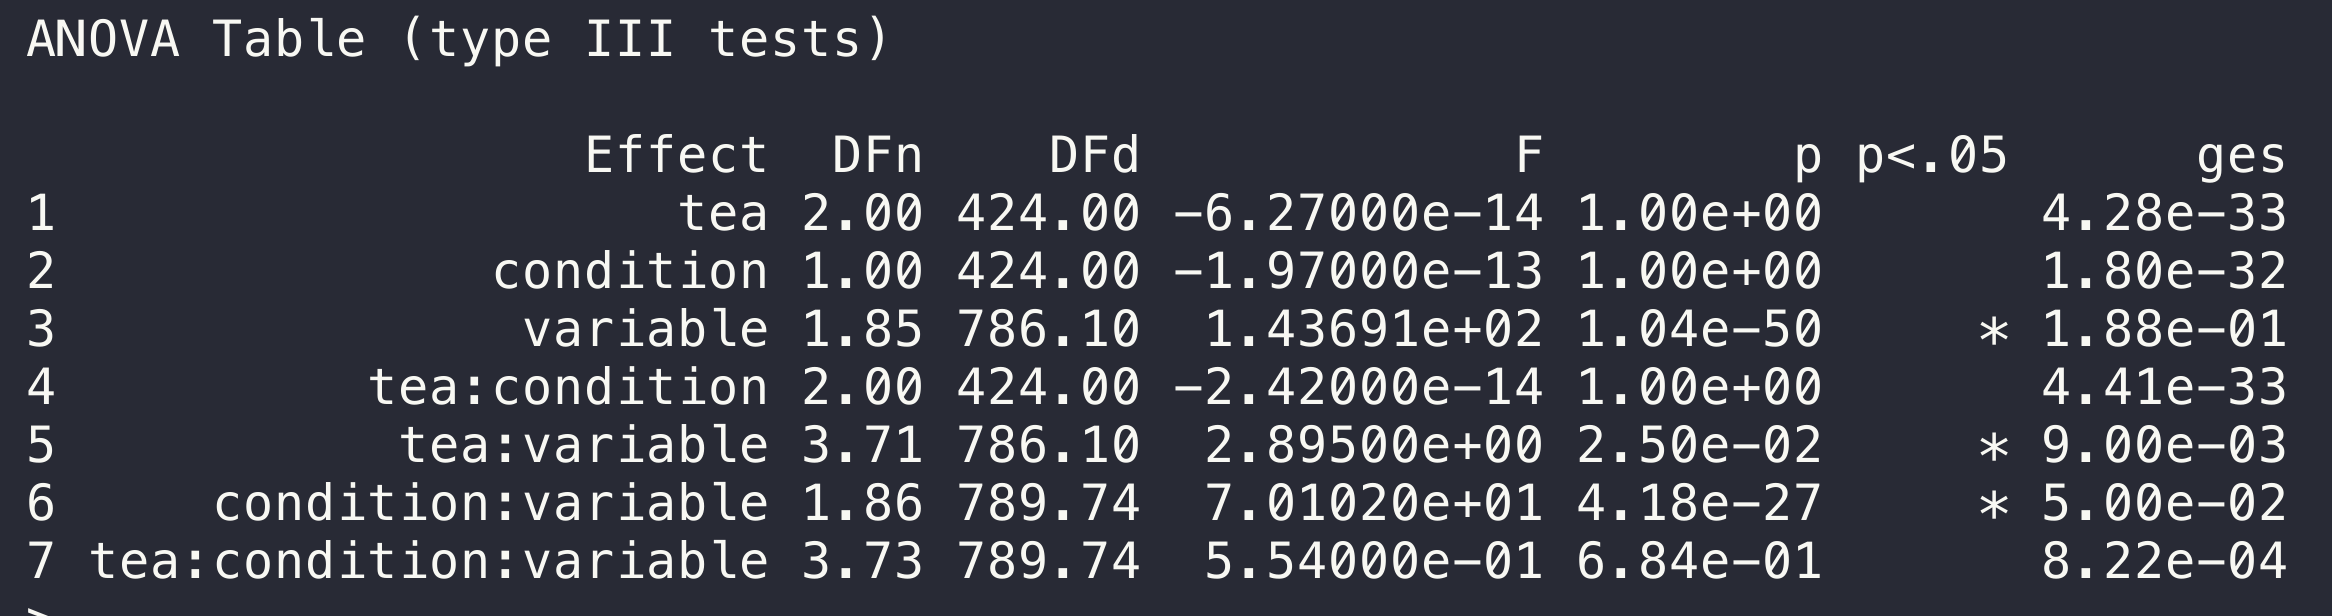
\includegraphics[scale=0.5]{./anovaProportion.png}}
  \centering
\end{figure}

\begin{figure}[H]
  \caption{Main effect of variable on proportion}
  \noindent\makebox[\textwidth]{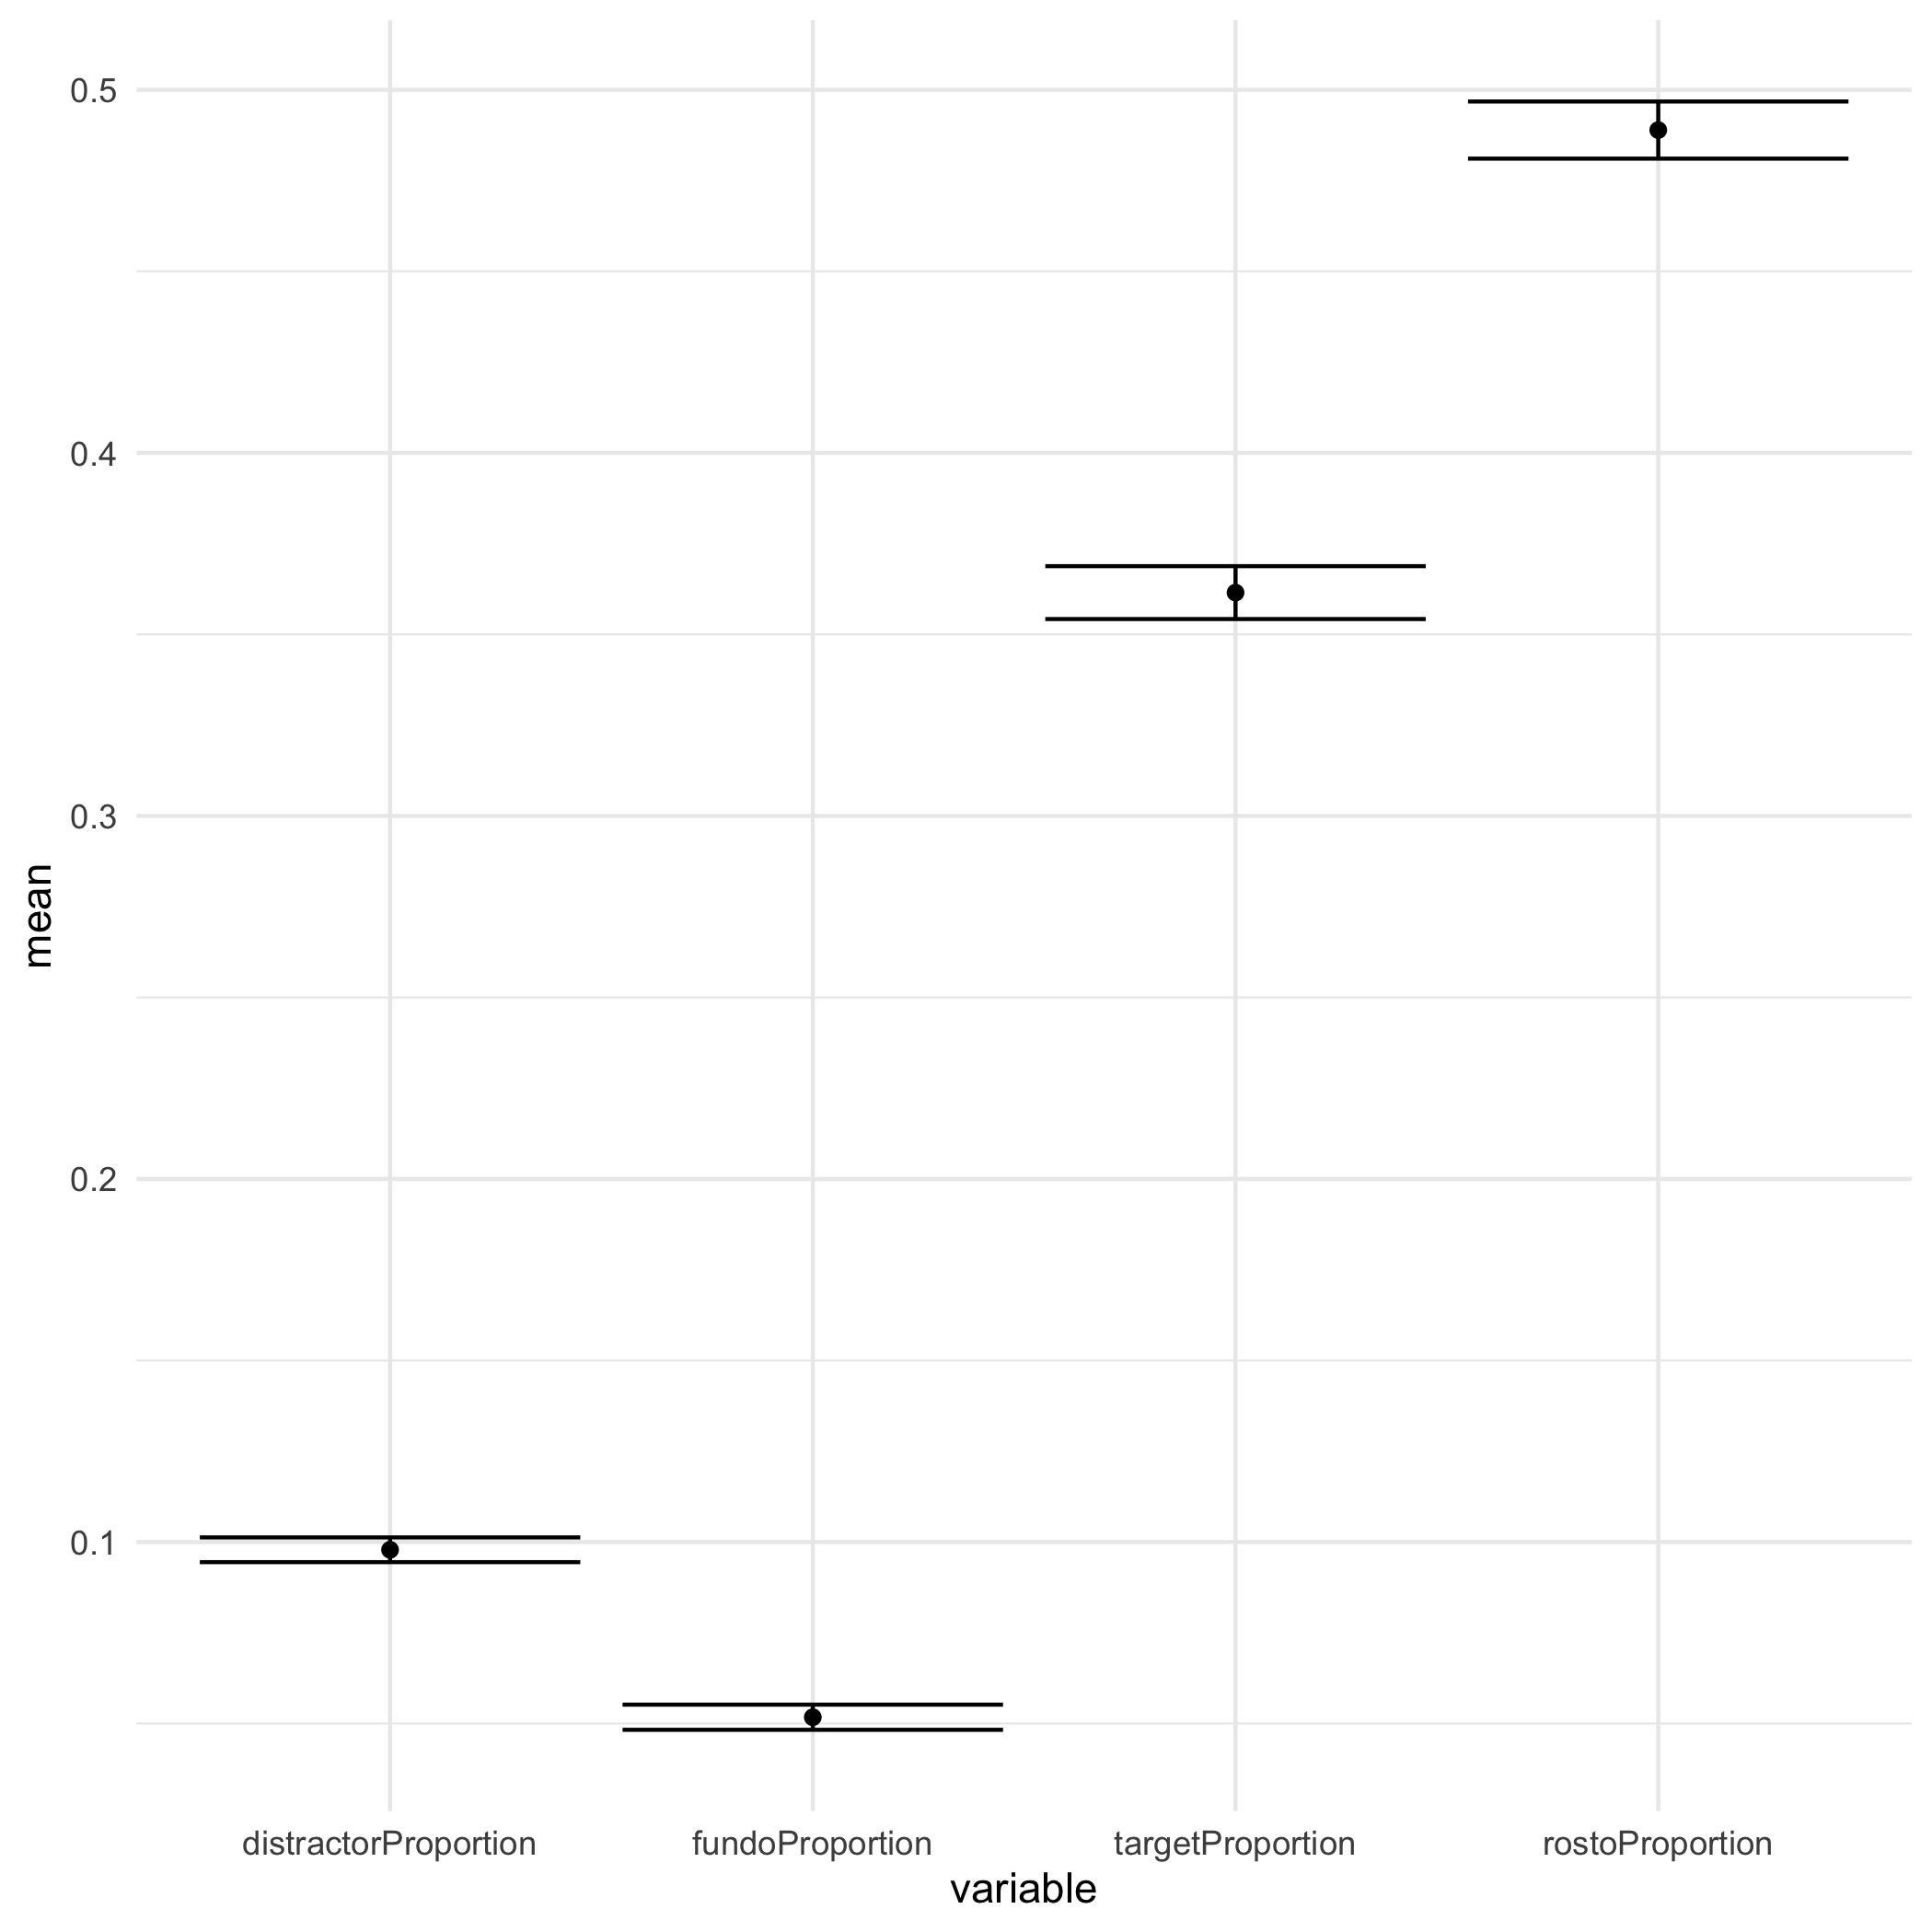
\includegraphics[scale=0.2]{./variableProportion.png}}
  \centering
\end{figure}

\begin{table}[ht]
\centering
\caption{Main effect of variable on proportion}
\begin{tabular}{rlrr}
  \hline
 & variable & mean & stder \\ 
  \hline
1 & distractorProportion & 0.10 & 0.00 \\ 
  2 & fundoProportion & 0.05 & 0.00 \\ 
  3 & targetProportion & 0.36 & 0.01 \\ 
  4 & rostoProportion & 0.49 & 0.01 \\ 
   \hline
\end{tabular}
\end{table}

\begin{figure}[H]
  \caption{Interaction of tea and variable on proportion}
  \noindent\makebox[\textwidth]{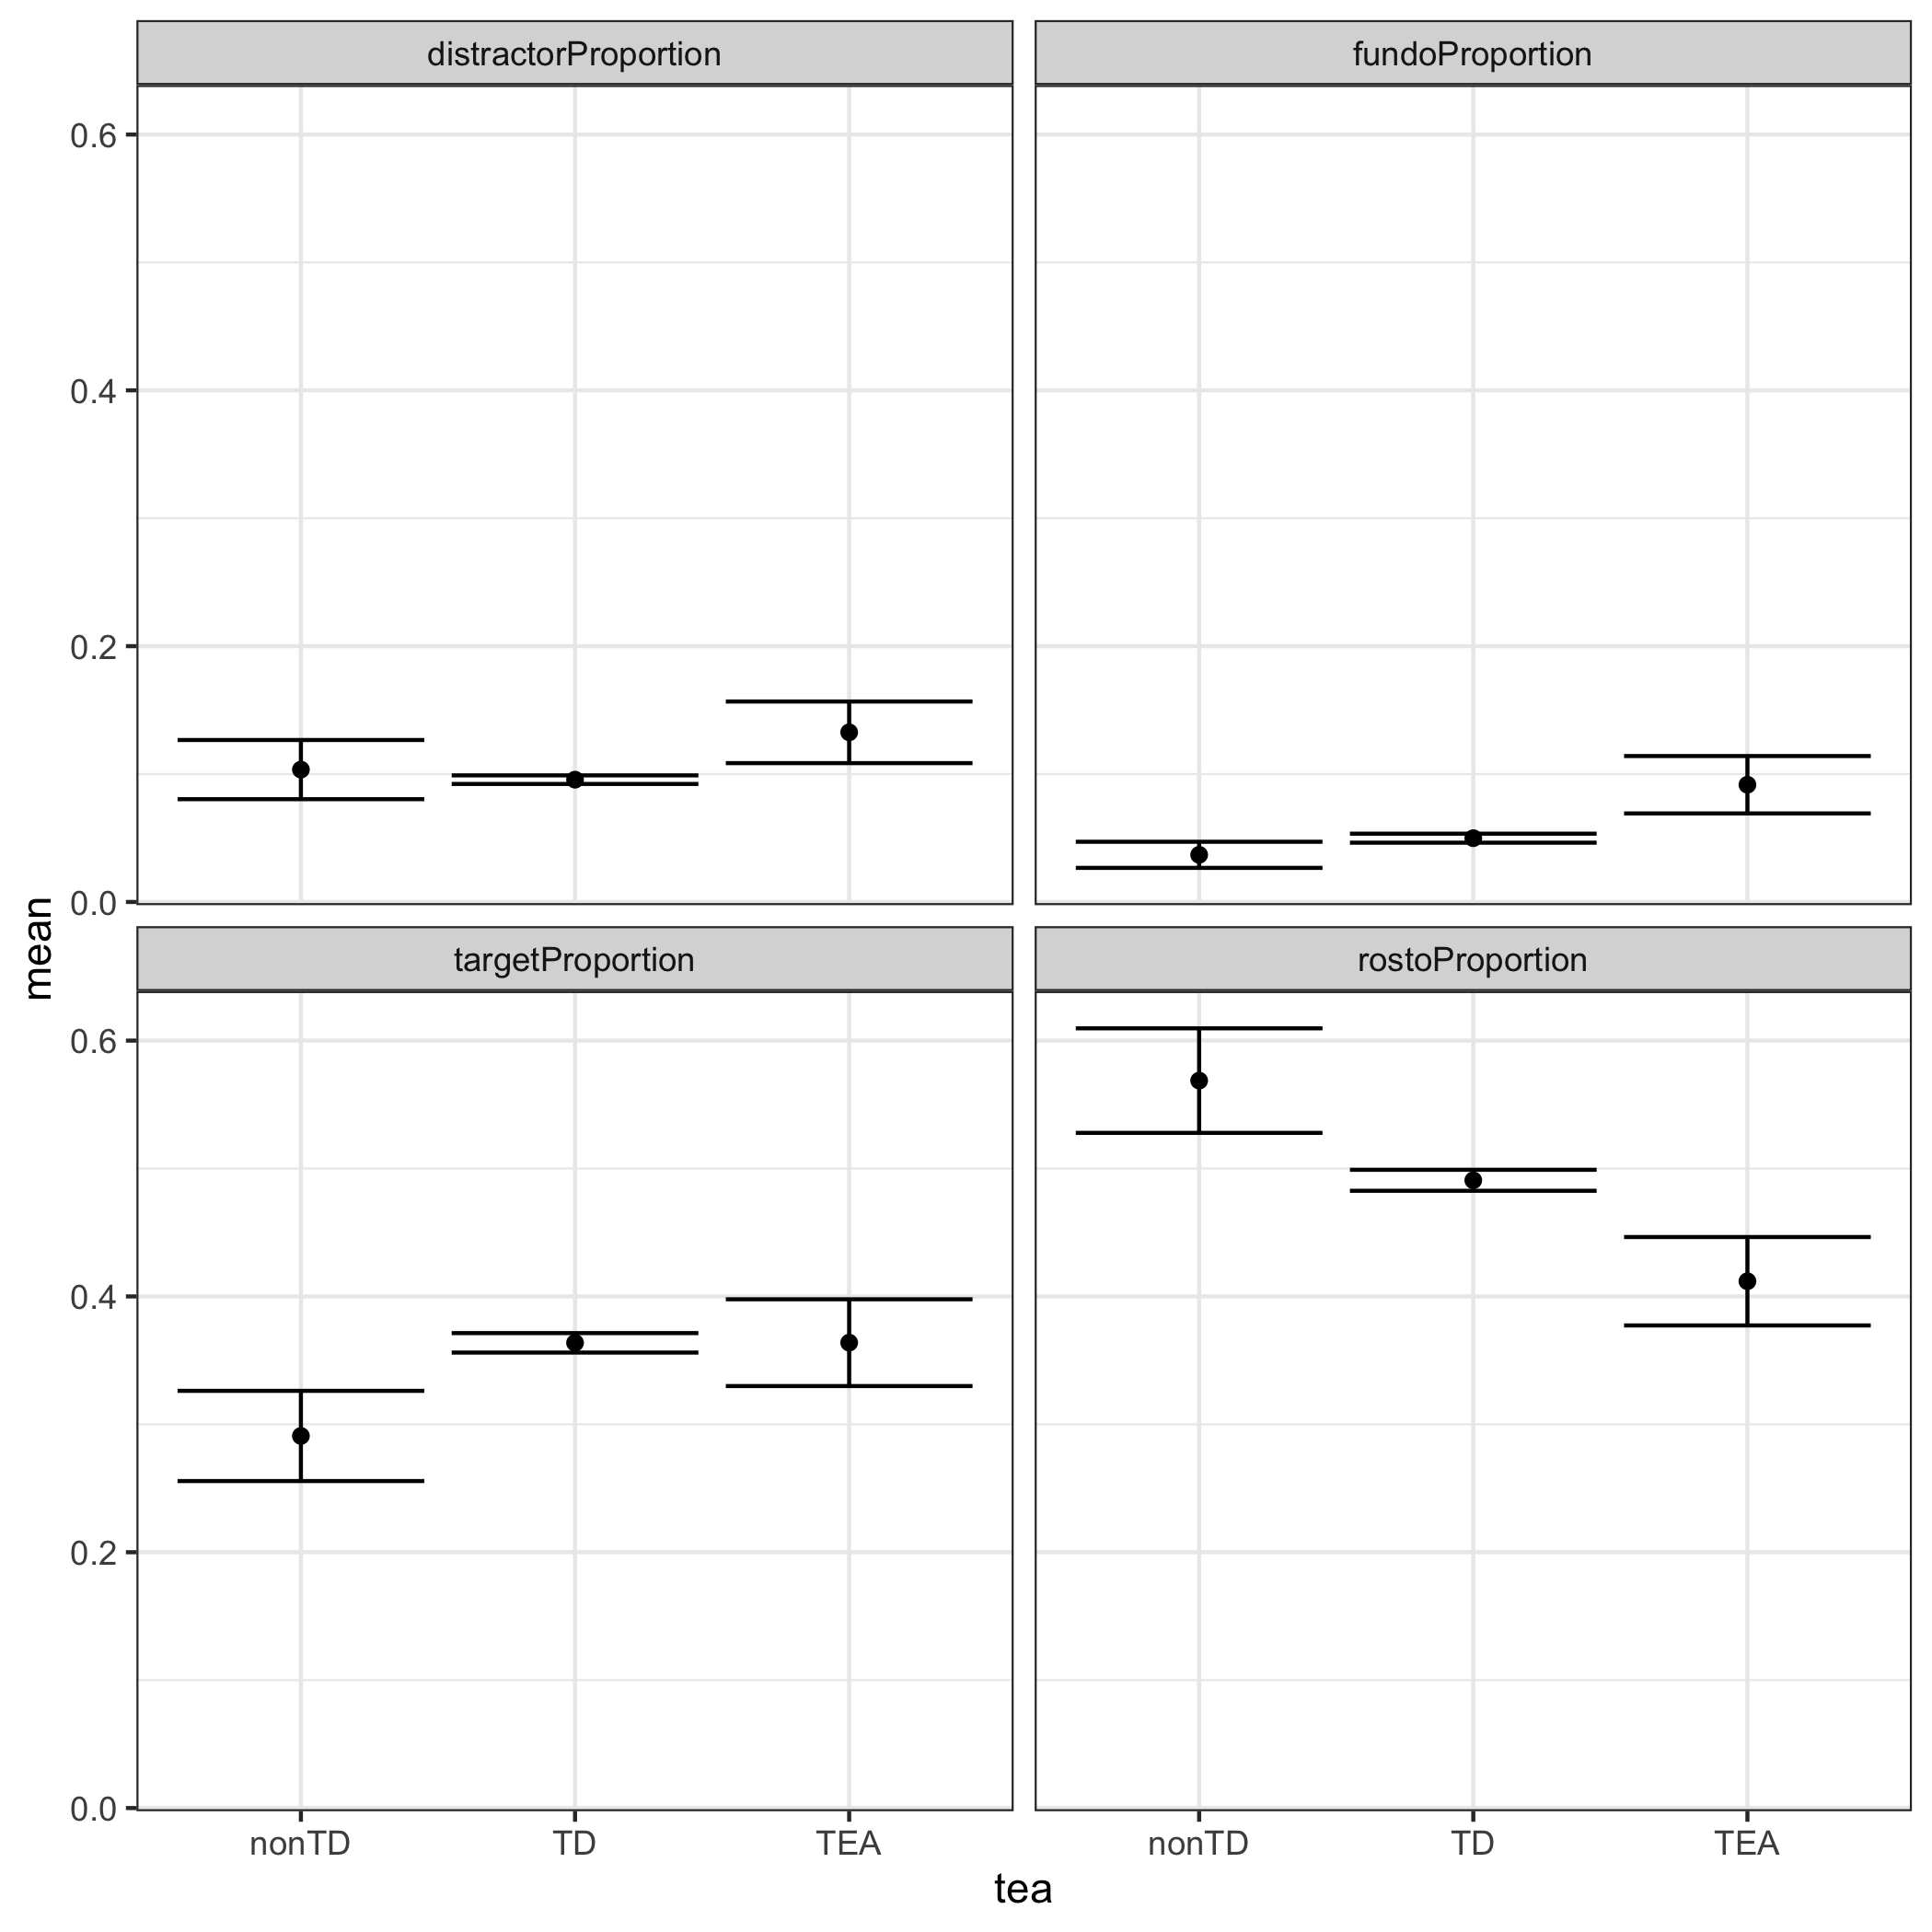
\includegraphics[scale=0.2]{./teaVariableProportion.png}}
  \centering
\end{figure}

\begin{table}[ht]
\centering
\caption{Interaction of variable and TEA on proportion}
\begin{tabular}{rllrr}
  \hline
 & variable & tea & mean & stder \\ 
  \hline
1 & distractorProportion & nonTD & 0.10 & 0.02 \\ 
  2 & distractorProportion & TD & 0.10 & 0.00 \\ 
  3 & distractorProportion & TEA & 0.13 & 0.02 \\ 
  4 & fundoProportion & nonTD & 0.04 & 0.01 \\ 
  5 & fundoProportion & TD & 0.05 & 0.00 \\ 
  6 & fundoProportion & TEA & 0.09 & 0.02 \\ 
  7 & targetProportion & nonTD & 0.29 & 0.04 \\ 
  8 & targetProportion & TD & 0.36 & 0.01 \\ 
  9 & targetProportion & TEA & 0.36 & 0.03 \\ 
  10 & rostoProportion & nonTD & 0.57 & 0.04 \\ 
  11 & rostoProportion & TD & 0.49 & 0.01 \\ 
  12 & rostoProportion & TEA & 0.41 & 0.03 \\ 
   \hline
\end{tabular}
\end{table}

\begin{figure}[H]
  \caption{Interaction of condition and variable on proportion}
  \noindent\makebox[\textwidth]{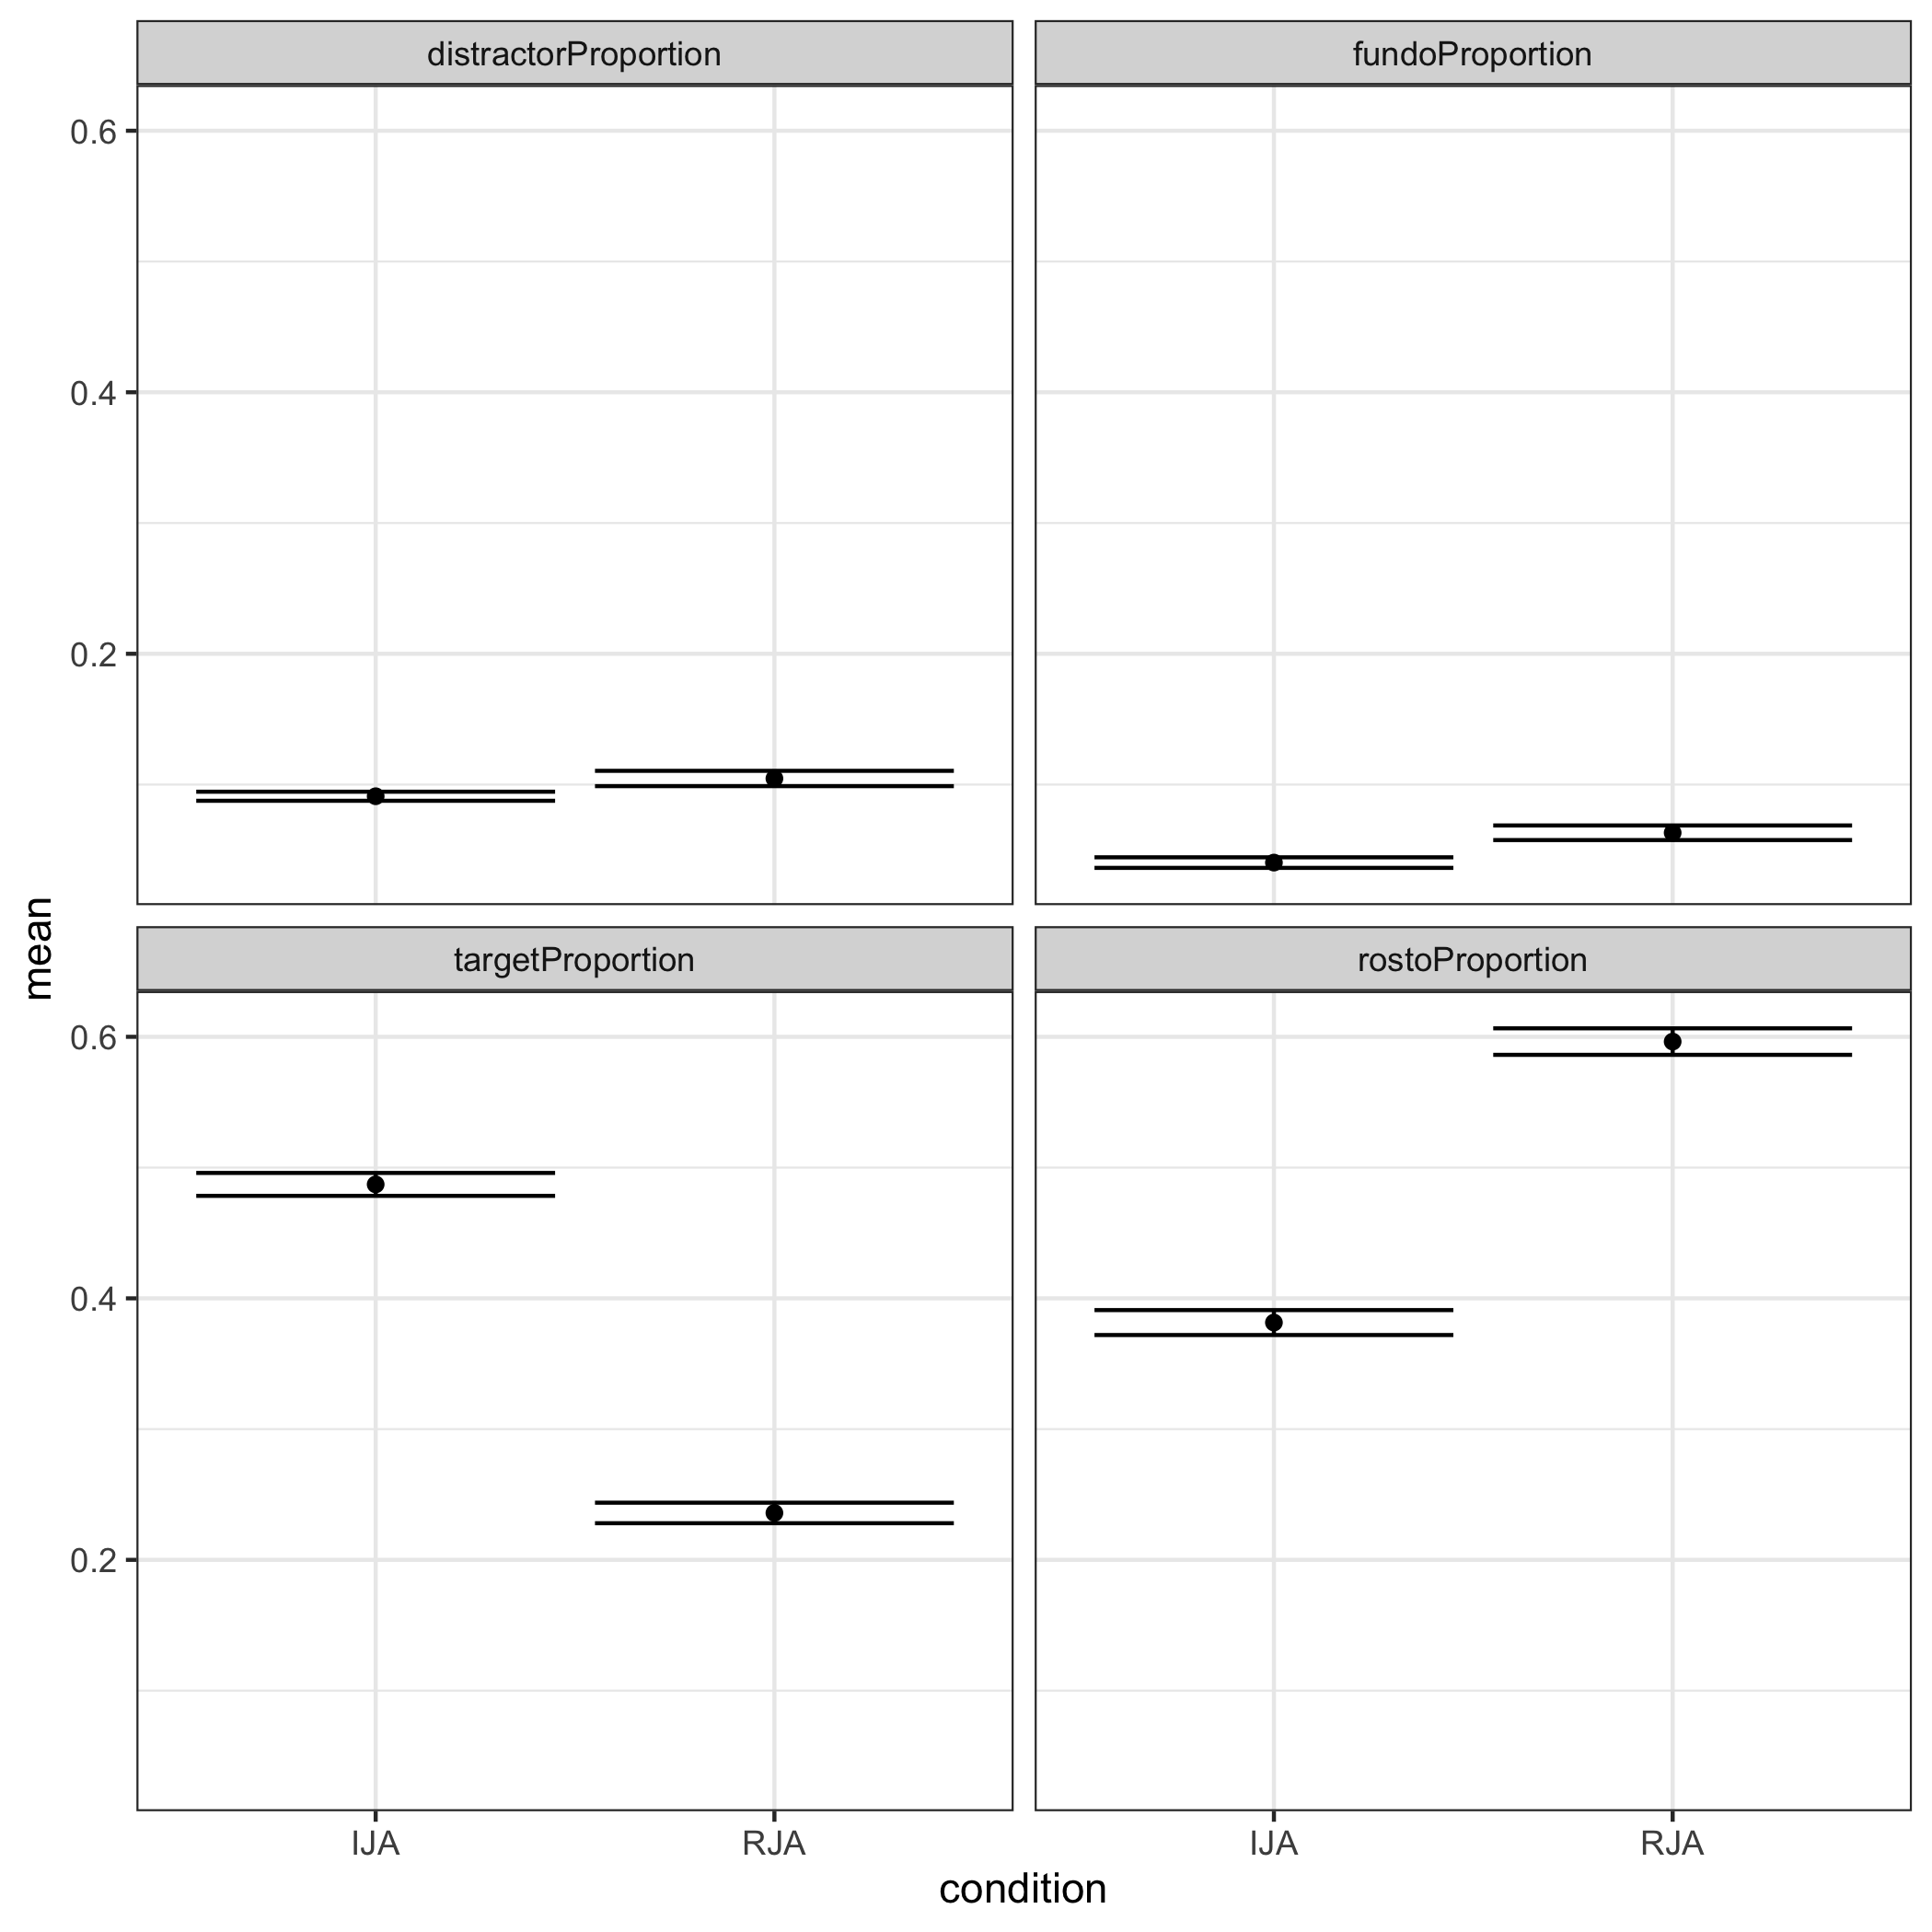
\includegraphics[scale=0.2]{./conditionVariableProportion.png}}
  \centering
\end{figure}

\begin{table}[ht]
\centering
\caption{Interaction of condition and variable on proportion}
\begin{tabular}{rllrr}
  \hline
 & condition & variable & mean & stder \\ 
  \hline
1 & IJA & distractorProportion & 0.09 & 0.00 \\ 
  2 & IJA & fundoProportion & 0.04 & 0.00 \\ 
  3 & IJA & targetProportion & 0.49 & 0.01 \\ 
  4 & IJA & rostoProportion & 0.38 & 0.01 \\ 
  5 & RJA & distractorProportion & 0.10 & 0.01 \\ 
  6 & RJA & fundoProportion & 0.06 & 0.01 \\ 
  7 & RJA & targetProportion & 0.24 & 0.01 \\ 
  8 & RJA & rostoProportion & 0.60 & 0.01 \\ 
   \hline
\end{tabular}
\end{table}

\begin{figure}[H]
  \caption{Interaction of condition, variable and TEA on proportion. *not statistically significant.}
  \noindent\makebox[\textwidth]{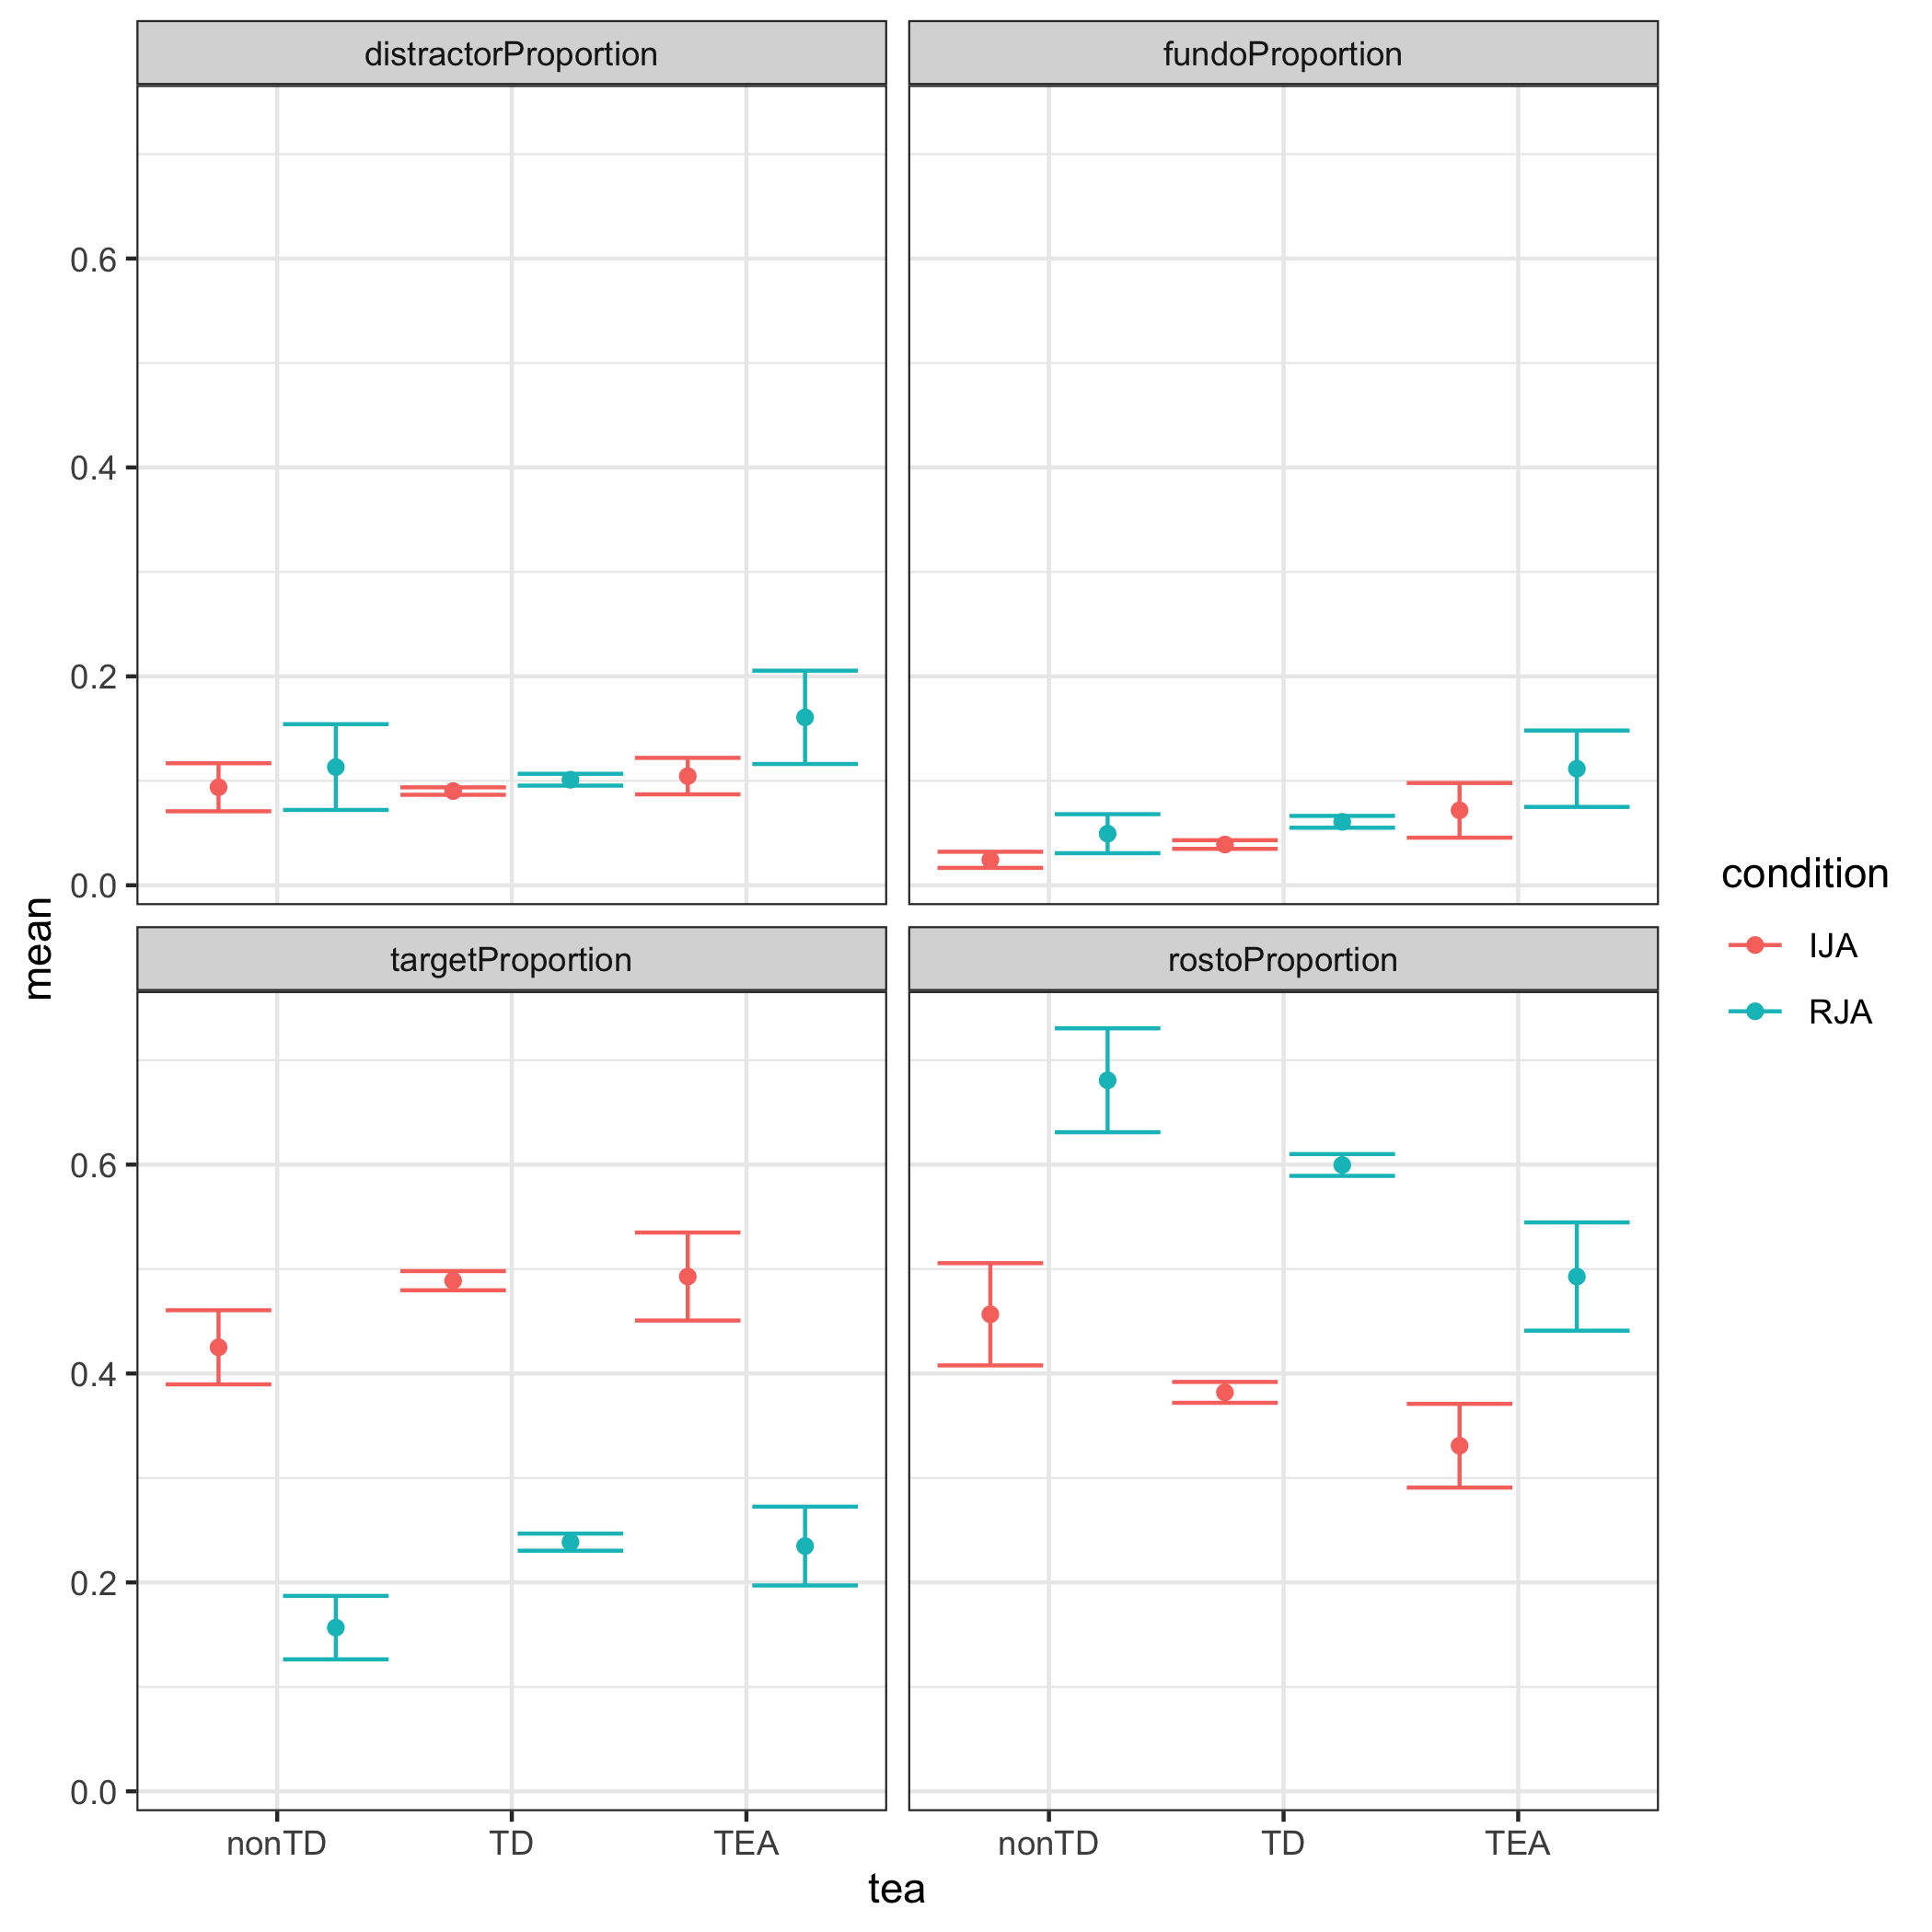
\includegraphics[scale=0.2]{./conditionVariableTEAProportion.png}}
  \centering
\end{figure}

\begin{table}[ht]
\centering
\caption{Interaction of condition, variable and TEA. *Not statistically significant.}
\begin{tabular}{rlllrr}
  \hline
 & condition & variable & tea & mean & stder \\ 
  \hline
1 & IJA & distractorProportion & nonTD & 0.09 & 0.02 \\ 
  2 & IJA & distractorProportion & TD & 0.09 & 0.00 \\ 
  3 & IJA & distractorProportion & TEA & 0.10 & 0.02 \\ 
  4 & IJA & fundoProportion & nonTD & 0.02 & 0.01 \\ 
  5 & IJA & fundoProportion & TD & 0.04 & 0.00 \\ 
  6 & IJA & fundoProportion & TEA & 0.07 & 0.03 \\ 
  7 & IJA & targetProportion & nonTD & 0.43 & 0.04 \\ 
  8 & IJA & targetProportion & TD & 0.49 & 0.01 \\ 
  9 & IJA & targetProportion & TEA & 0.49 & 0.04 \\ 
  10 & IJA & rostoProportion & nonTD & 0.46 & 0.05 \\ 
  11 & IJA & rostoProportion & TD & 0.38 & 0.01 \\ 
  12 & IJA & rostoProportion & TEA & 0.33 & 0.04 \\ 
  13 & RJA & distractorProportion & nonTD & 0.11 & 0.04 \\ 
  14 & RJA & distractorProportion & TD & 0.10 & 0.01 \\ 
  15 & RJA & distractorProportion & TEA & 0.16 & 0.04 \\ 
  16 & RJA & fundoProportion & nonTD & 0.05 & 0.02 \\ 
  17 & RJA & fundoProportion & TD & 0.06 & 0.01 \\ 
  18 & RJA & fundoProportion & TEA & 0.11 & 0.04 \\ 
  19 & RJA & targetProportion & nonTD & 0.16 & 0.03 \\ 
  20 & RJA & targetProportion & TD & 0.24 & 0.01 \\ 
  21 & RJA & targetProportion & TEA & 0.23 & 0.04 \\ 
  22 & RJA & rostoProportion & nonTD & 0.68 & 0.05 \\ 
  23 & RJA & rostoProportion & TD & 0.60 & 0.01 \\ 
  24 & RJA & rostoProportion & TEA & 0.49 & 0.05 \\ 
   \hline
\end{tabular}
\end{table}
\end{document}
